\chapter{Using time feedback to manage interruptions}\label{ch:56}
\begin{mynote}
\subsubsection{Chapter outline}
This chapter describes two studies that evaluate whether giving people feedback on the duration of inquiries can influence people's switching strategies and data entry performance. A browser notification was developed which showed people how long they switch away for on average. Study 6 evaluated the notification with an experimental task to measure switching behaviour and task performance. Study 7 evaluated the notification in the office setting with workers doing data entry work, to ascertain how appropriate the proposed recommendations are for a naturalistic task.

Together these studies show that time feedback can reduce the duration of inquiries, making participants faster and more accurate in completing data entry tasks.  
\end{mynote}

\section{Introduction}
The studies reported in this thesis so far have shown that people adopt different strategies to manage inquiries, given the time costs associated with these different inquiries. Office workers in Study 2 postponed physical interruptions if they took time, or prepared physical information sources beforehand. Digital interruptions however were addressed immediately as participants presumed them to be quick, which suggests that people are not aware of the time these interruptions actually take: participants were commonly observed being distracted and getting logged out of the data entry system for being away for too long. The experimental studies in Chapter 4 showed that if participants learn the time it takes to make a digital interruption, they postpone addressing inquiries with a high time cost and enter other information first. The problem is that outside of a controlled setting, it is difficult to know how long a digital interruption may actually take. People do not always know where to get information from, may get distracted, or can further self-interrupt to other tasks. How can people be better supported in managing these inquiries with unknown time costs?

Based on the thesis findings so far and prior literature on interruption and information management tools, this chapter presents a design intervention which shows how long people go away from their data entry work. The intervention was evaluated in an online experiment and field study, to investigate whether time feedback can not only help postpone long inquiries, but also reduce the number and duration of inquiries and improve people’s focus during data entry work. Before presenting the intervention, prior work on information and interruption management tools are reviewed. 

\subsection{Delaying the intention to interrupt}
The timing of an interruption matters, and it is better to defer an interruption at a more convenient moment in the task. For example, it is less disruptive to interrupt a task at a low-workload than high-workload moment \citep{Gould2013a, Iqbal2005}. Prior studies have shown that people choose to defer interruptions until low workload moments if given the option to do so, and if they do not have to hold the intention to interrupt in memory \citep{Gilbert2015, Salvucci2010}. \citet{Gilbert2015} looked at people’s off-loading behaviour of future tasks in both an experimental and naturalistic setting. Participants had to remember to perform an action later, and had the option to offload this intention or to keep it in memory. In both settings, a majority of participants offloaded these intentions when they had the option, and this significantly improved their task performance. Additionally, in Study 3 of this thesis, where participants had to copy a block pattern and remember which blocks to drag to which location, a selection of participants placed blocks nearby what they though the correct location was, to not have to remember its location, and as a reminder to place them there later. 

These findings suggest that if people have to memorise which information to retrieve, they may benefit from options to offload these information needs, and are able to effectively defer inquiries until a convenient moment in the main data entry task. However, there is also time effort involved in offloading information, and the time it takes to offload is only worthwhile if it is outweighed by the time it takes to address the interruption. If people are not aware how long an inquiry will take, as was observed in Study 2, there may be little incentive to offload and delay these inquiries: it is presumed to be faster to address the interruption immediately.

\subsection{Improving information search}
The duration of an interruption matters as well: the longer it is, the more disruptive it is \citep{Altmann2017, Monk2008}. Inquiries may take time  if information is scattered across documents and applications, and users have to go in and out of these separately to search and find what they are looking for. To shorten the time it takes to find information across applications, \citet{Dumais2003} developed Stuff I’ve Seen, a unified search interface which allows users to search through information they had already seen before across applications, such as emails, documents and web pages. A user study found that participants rather used the tool than individual search tools of each application. However, searching for information was not the only type of time cost found in Chapter 3: sometimes participants were quick to find the information source they were looking for, but were distracted by other information. Information search tools are therefore insufficient to reduce the duration of these inquiries. 

\subsection{Preparing task information}
Lastly, while some interruptions can be beneficial, all interruptions may become disruptive if they happen too often.The number of inquiries may be decreased if people organise information to have it nearby during the task. People already displayed this behaviour somewhat in Study 2 by collecting physical information they knew they were going to need nearby, to make it easier to access. Some tools have looked at making digital information easier to access during a task as well. For example, GroupBar \citet{Smith2003} allows users to group windows needed for a task in the task bar. This can be particularly useful when resuming an interrupted task: the user can see which documents were used before leaving the task. Similarly, Microsoft Office’s new feature TAP \footnote{https://support.office.com/en-gb/article/Find-and-use-the-content-you-need-when-you-need-without-leaving-Word-860118fc-1f61-41f6-922f-40084a284658} allows users to place relevant documents in a task pane next to their working document. The aim of the feature is to keep focus on document creation, rather than looking up information. The feature is presented as a task pane within a document, such as a text document or email, and contains an overview of documents that may be relevant to the current document. These tools are mainly focused on re-using content from archived documents, and assumes the user knows which documents to re-use. The tools provide less support for a new activity in which new sources need to be accessed. 

\subsection{Feedback to improve task performance}
An alternative approach is to give people information about their task strategies, as giving people feedback can help them in improving their performance on a task \citep{Maior2018, Farmer2017}. The findings in this thesis so far suggest that people can be good at managing interruptions, if they are aware of the time costs. Could people therefore improve how they manage digital interruptions if they are shown the time costs associated with digital interruptions? 

Giving users feedback on time spent on digital activities has been utilised by a series of time and interruption management tools before \citep{Lyngs2018}. The primary aim of these tools is to support users in self-regulating their ICT use and making more effective use of their time. Commercial applications such as RescueTime and ManicTime provide users an overview of their computer activities, to reflect how much they spend in total on certain sources. These applications show people’s entire computer usage, and interview studies revealed it is often not clear to users what to do with this data \citep{Collins2014}. Furthermore, a problem with retrospective information is that it lacks context, and users have to remind themselves to look at it \citep{Whittaker2016}. On the other hand, feedback which is given during a task allows users to apply the information immediately on the current task they are working on \citep{Gould2016a, Maior2018}. \citet{Gould2016a} looked at switching behaviour during online crowdsourcing work, and found that an intervention during work that encouraged people to stay focused after they had self-interrupted reduced the number of switches to unrelated tasks. \citet{Whittaker2016} interviewed office workers and students to establish user requirements for a time awareness application, and found users were primarily interested in their current activities rather than long-term behaviour. They developed and evaluated an application which presented users with a visualisation of the last 30 minutes of computer activity. The application reduced the time spent on non work-related activities such as social media, but it did not increase time spent on work. While these tools have shown how feedback during a task can reduce task-irrelevant interruptions, the effect of time feedback on managing work-related interruptions has been unexplored.

In summary, prior research has shown that people adapt to feedback given in the moment to improve performance on their task. My studies found that people adapt to time costs of inquiries in a controlled setting (Chapter 4), but are not aware of time costs of inquiries in an office setting, due to distractions, switching documents, and task-irrelevant information (Chapter 3). This chapter explores whether a design intervention which gives feedback on the duration of interruptions can help people manage these interruptions.

\section{Design process of developing the intervention}
%NOT FINISHED, PROOFREAD AND EDIT
The findings of Study 1 to 5 were used to produce initial design ideas for a design intervention. The main purpose at this ideation stage was to explore different approaches to support people in managing inquiries with unknown time costs. Sketches were made to investigate what the interaction would look like for these different ideas, and if they were deemed an appropriate tool to address the issues found in the studies. The final idea was chosen to develop further as the final intervention, and the other ideas were not developed further beyond sketches. The process resulted in four ideas: the first three ideas are presented and described briefly below. The final design intervention is discussed in more detail. 

\subsection{Idea 1: To do list}
The first idea considers a task pane embedded in the data entry interface (see Figure \ref{fig:ch56_Idea1}), that enables users to write down the inquiries that are needed as part of a task. As was found in Study 1 and 2, people may not always know they need information until they have already started a task. Rather than interrupting a task to look up information straight away, the to-do list enables people to set a reminder to look this up later at a more convenient moment in the task. Users have the freedom to decide to look information up themselves when they want, from both digital and non-digital sources.

A to-do list requires people to spend time writing down the intention to interrupt, and they still have to switch away from the data entry interface to look up information. Furthermore, people may not make the effort to write it down if the interruption is presumed to be short. 

\begin{figure}
\centering
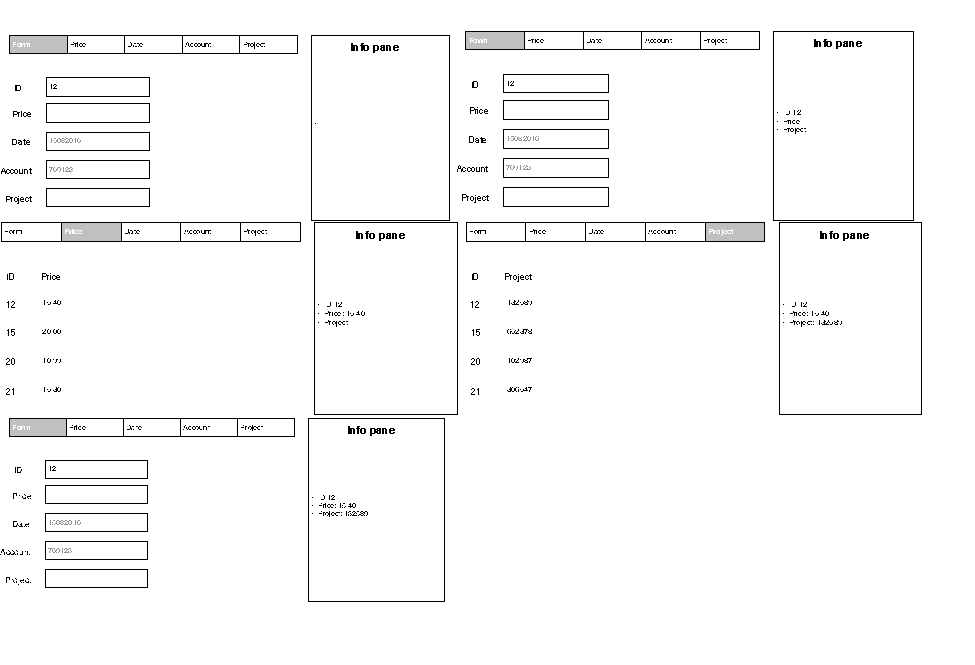
\includegraphics[width=\textwidth]{images/ch56/ch56_Idea1.pdf}
\caption{Idea 1 enables users to write down inquiries needed for the task, so they address these later at a more convenient moment in the task.}
%\vspace{-3pt}
\label{fig:ch56_Idea1}
\end{figure}

\subsection{Idea 2: pinboard}
The idea of a pinboard extends the first idea of a to-do list. The pinboard not only allows people to write down inquiries, but also enables the user to place the information in the task pane, once it has been retrieved (see Figure \ref{fig:ch56_Idea2}). 
Once they have found information, they can ‘pin’ this information source on their board, so if they need it to re-use this information again for future data entry tasks, they can look it up from the task pane and do not have to leave the interface and search for it again.

The information pane to pin and write down information is embedded in the main task interface, so the user does not have to switch to a separate application to search or view information, and the information is at hand when needed. 

\begin{figure}
\centering
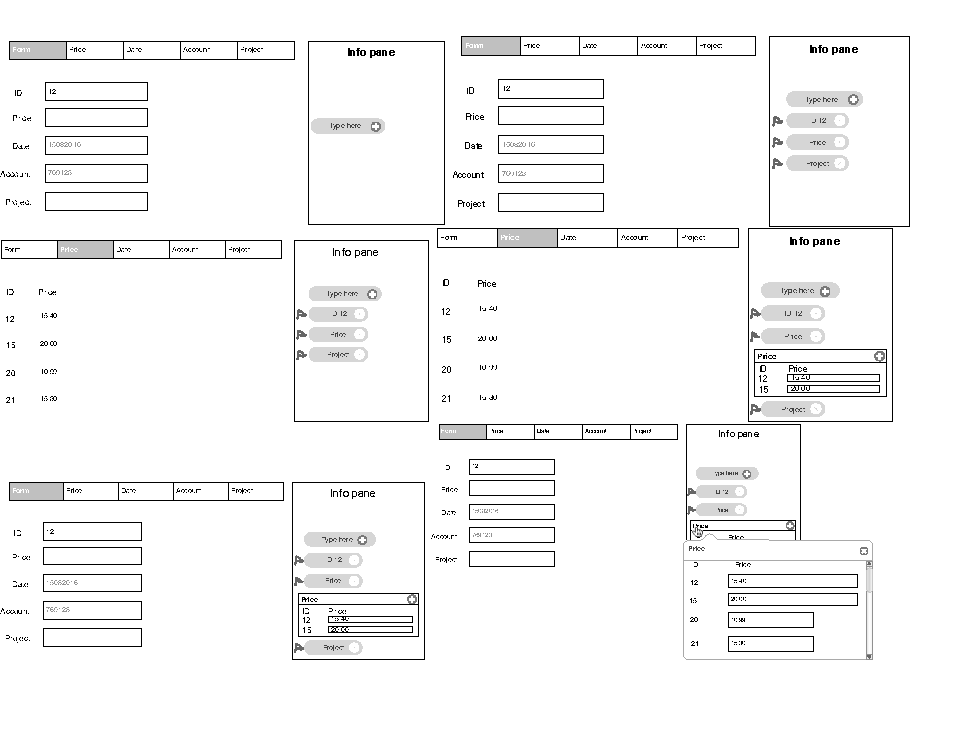
\includegraphics[width=\textwidth]{images/ch56/ch56_Idea2.pdf}
\caption{Idea 2 enables users to pin information in the task pane, so information is at hand if it needs to be re-used in the future.}
%\vspace{-3pt}
\label{fig:ch56_Idea2}
\end{figure}


\subsection{Idea 3: search function}
The search function revolves around the idea of minimising the time spent away from a task interface to look for information. A search function allows users to search within the task pane for new information (see Figure \ref{fig:ch56_Idea3}). 
A snippet of search results is shown in the task pane, and the user can click on one of the search results to expand the information source and view the information.

\begin{figure}
\centering
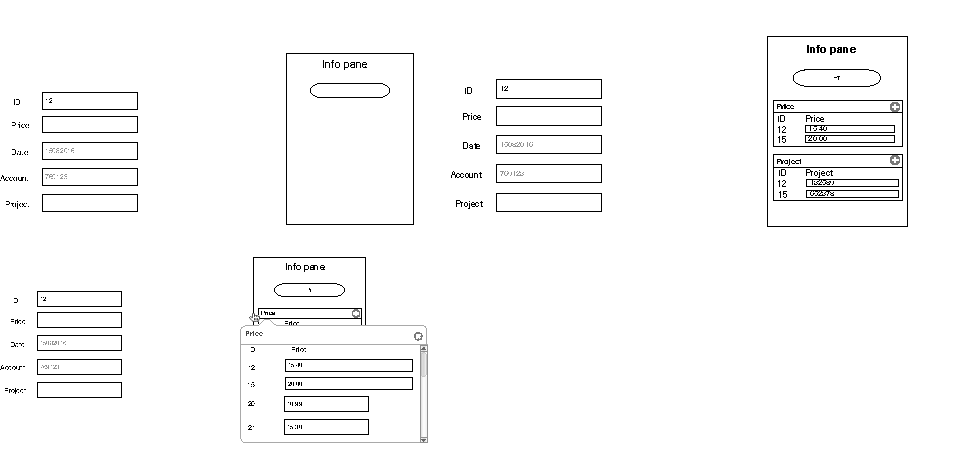
\includegraphics[width=\textwidth]{images/ch56/ch56_Idea3.pdf}
\caption{Idea 2 enables users to search for information in a task pane, without leaving the main task interface.}
%\vspace{-3pt}
\label{fig:ch56_Idea3}
\end{figure}

\subsection{Idea 4: Time feedback}
The first three ideas revolved around reducing the number or duration of people’s interruptions. However, these ideas would not necessarily make people more aware of the time they spend on interruptions, which was found to be a potential issue in Study 2. Upon reflection on these ideas, I was uncertain whether people would be willing to invest time in using a tool, if they would still be under the impression that their interruptions were short and not disruptive. 
I therefore focused on developing a design intervention that would also make people more aware of time costs of interruptions, and whether this increased awareness would encourage people to reduce the number and duration of interruptions themselves. To increase awareness, the idea of a notification was developed that would give people feedback on their interruption behaviour. The notification gave information about the time people spent on interruptions, to see whether showing this information would reduce the duration and number of interruptions.

\subsubsection{The moment of feedback}
A first design consideration in developing the intervention was how the information should be presented to the user. Previous research found that users find it difficult to put reflective information about their use of time into context \citep{Collins2014, Whittaker2016}. Instead, giving feedback about task performance during a task has been shown to make users adjust their task strategies in the moment \citep{Maior2018, Gould2016a, Whittaker2016}. It was therefore decided that, for the information to be most effective, it should appear during a task. To make people more aware of their interruptions, information is shown upon every interruption away from a primary task. 
A second consideration was at which moment of an interruption the information should be shown: before or after an interruption. It was decided to show the information at the start of an interruption, so the user would be able to apply potential adjustments to their interruption behaviour immediately for that particular interruption. If information had been shown after an interruption, the interruption would have already taken place, and the user would have to remember to change their behaviour for future interruptions.

\subsubsection{The type of time feedback}
As the information is shown at the start of an interruption, it is difficult to provide any accurate information about the exact duration of the interruption that is about to take place. Therefore, the intervention shows the average interruption time of all previous interruptions, to give an indication how long the interruption could take, based on past behaviour. The intervention considers the average time of all digital interruptions away from a specific task, that is when the user switches from a specific task to another computer window. 

The intervention considers the time of an interruption overall, and not just time spent in a particular application or website the user switches to. Even though interruptions may be expected to take longer if the user switches to a distracting source, the user may visit several windows during an interruption before returning to the task, behaviour which was commonly observed in Study 2. The time spent in a specific source may therefore not give an accurate picture of the overall duration of interruptions, as people may only stay in the first window for a short time but the overall interruption may take much longer. 

\subsubsection{Task sequence}
The information was presented to the user through a notification. Figure 4 shows what the interaction with the design intervention would look like. Step 1 shows the window of an expenses task the user has to complete. To complete this type of task, information needs to be retrieved by switching to another window (Step 2). Upon every switch away from the task interface, a notification appears telling the user how long these switches are on average. If the user switches for the first time, the notification says that no data is available yet to give an average time. Once the right information has been found, the user then has to switch back and enter this information in the correct field (Step 3). 

\begin{figure}
\centering
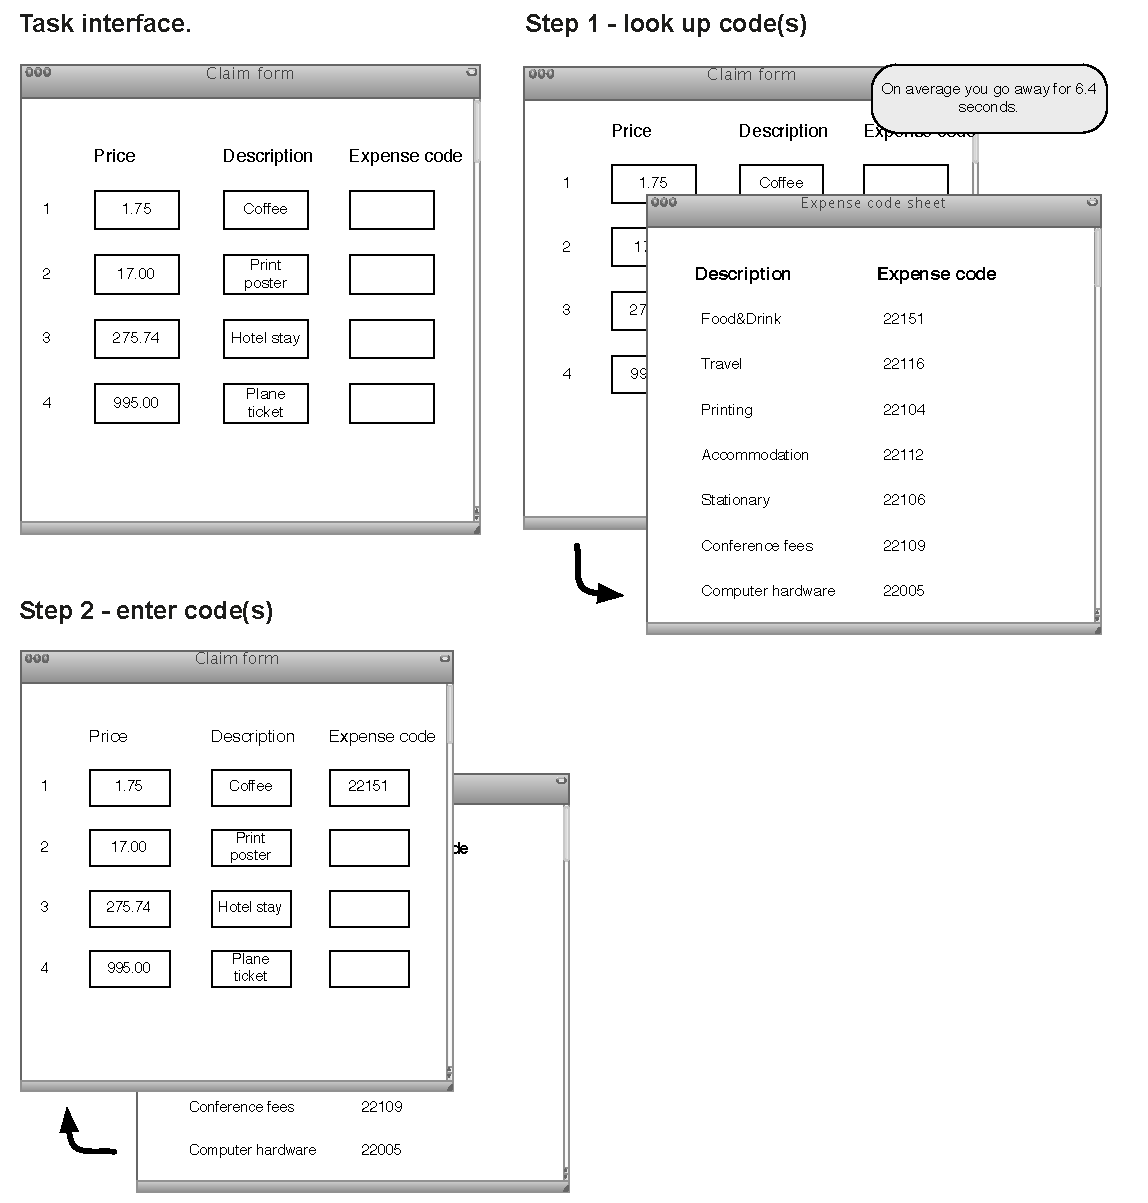
\includegraphics[width=\textwidth]{images/ch56/ch56-wireframe.pdf}
\caption[Wireframe of the design intervention.]{A wireframe to indicate what the interaction with the intervention will look like. The upperleft corner shows the window of an expenses task the user has to complete. Information for this task is retrieved by switching to another window (Step 1). Upon every switch, a notification appears telling the user how long these switches are on average. The user then has to switch back and enter this information in the correct field (Step 2). Step 1 and 2 are repeated until all codes have been entered; the user can switch back and forth as often as is needed.}
%\vspace{-3pt}
\label{fig:ch56-6_Wireframe}
\end{figure}

\subsection{Implementation}
The intervention was implemented as a browser notification. As was found in Chapter 3, participants’ data entry work was conducted in a web browser and revolved around a main data entry web page. Every switch between the task page and another computer window, such as another browser window or a different application, was recorded to calculate the number and duration of switches. The browser notification used this data to show users the average time of their interruptions. 

The notification was evaluated in an online experiment in Study 6, and in an office workplace in Study 7. The visual presentation of the notification to participants was the same in both studies, but because of the different study environments, the implementation differed slightly between studies. In Study 6, the browser notification was implemented in the experimental data entry interface. In Study 7, the browser notification was implemented as a browser extension that the participants could install on their own computer and use on any website they wanted. The implementation details are further discussed in the separate study sections. The notification was evaluated in a pilot study with colleagues before using it in the studies. 

\section{Study 6: Looking up information in email during an online experiment}\label{st:Study6}
\textit{This study and early results have been published in \citet{Borghouts2018a} and were presented at the CHI conference in 2018.}

\subsection{Introduction}
%BRIDGE WITH LAST CHAPTER
\begin{comment}
The findings of the previous studies will have given insight into the influence of IAC on people's strategies of managing looking up information and how different strategies may be more efficient and accurate than others. For example, one finding can be that people who look up information from high IAC sources as they need it are slower and make more data entry errors than people who first collect all information and then enter it all in one sequence. 
It will have highlighted some functionalities that a data entry expenses system needs to offer users. These findings are translated into a set of requirements. These are used to test the existing system against, and used to develop possible future design recommendations suited to the task of entering expenses. 

The design recommendations will take into account both findings from Study 3 and 4 on what influences people's strategies and what is desirable, as well as the setting studied in Study 1 and 2 and what is feasible. For example, desired changes in the actual interface may be too expensive to be realistic, and it may be more feasible to change the way information sources are designed, or how these are laid out in the user's environment. Screenshots of the current interface system will be used (initial ones were obtained in Study 1, additional ones will be obtained in Study 2). 

Study 5 aims to test different designs in a controlled experiment, to investigate if changing design features influences people's switching strategies and their speed and accuracy in data entry. It will use the same task paradigm as Study 4 and compare different designs, to see if these changes have an influence on the strategies people adopt in looking up information for a data entry task, and whether these changes can make people adopt strategies that improve accuracy. 

Observations in Study 2 showed that data workers prepare some information they need for a data entry task beforehand. Other data items are retrieved as the task goes along. As soon as they realise they need information, they interrupt themselves and this can happen frequently during a single task. Finding information can take longer than expected, and people can get distracted along the way. In general, finding information is disruptive: people may forgotten where they were in a task, enter information in the wrong fields, or they might be automatically logged out of a system because of inactivity. Study 4 and 5 showed that in a controlled setting where people know the time it will take them to retrieve information, they adapt and schedule their tasks accordingly. They will look up and enter items that take the least time first, and postpone getting information that is difficult to lookup. An issue is that people often do not know how long it will take them and therefore cannot schedule or adapt to it. Can people be nudged into making more mindful interruptions, if they are given feedback on how long it takes them to find information?

A number of laboratory studies have looked at how people decide when to address interruptions. These studies showed that people defer interruptions until lower workload moments \citep{Salvucci2010}, or switch to another task when there is a delay in the primary task \citep{Gould2016, Katidioti2013}. However, these studies primarily focused on characteristics of the primary task, and it is unclear from these studies if the time taken to address an interruption has any effect. Study 4 and 5 showed that if the time to access data items for a data entry task is consistent throughout a controlled experiment, participants learn to look up and enter easy-to-access items first, before looking up other items. Might people therefore manage their interruptions differently, if they are given feedback on how long it takes them to find information?

\citet{Gould2016a} looked at people's switches to other, unrelated activities during an online routine data entry task. They found that a cue that asked participants to remain focused on the task after they switched reduced self-interruptions. The aim of the two studies in the current chapter was to see if a cue which indicates the duration of an interruption has any effect on people's switches to a related activity: look up information for a data entry task. Study 6 used an experimental data entry task to measure if a notification showing the average duration on people's switches had an effect on number and duration of their switches, and data entry speed and accuracy. Study 7 evaluated the feedback with data workers doing expenses work, to evaluate if the notification would be suitable for an applied task.

\end{comment}

%INTRODUCTION TO CURRENT
This study aimed to investigate whether an intervention showing people how long they switch on average reduces the duration and number of switches during a data entry task. An online experiment was conducted where participants had to complete a data entry task. Participants had to enter numeric codes into a form, which they had to retrieve from a message sent to their personal email. The information was presented as a message in participants' email inboxes, as email is an integral part of data entry work but known to be a source of distraction, and people often spend more time on it than originally intended \citep{Hanrahan2015, Mark2016}. It was therefore expected to have a distracting effect during the switches to look up information. Half of the participants received feedback on the average length of their switches through a browser notification. 
This study aims to investigate whether time feedback on interruption length reduces the number of switches, reduces the duration of switches, makes people faster in data entry, and makes people more accurate in data entry.

\subsection{Method}
\subsubsection{Participants}
Fourty-seven participants (30 women) took part in the online experiment. Ages ranged from 20 to 63 (M = 29.3 years, SD = 9.1 years). The participants were recruited via university email lists, social media and online platforms to advertise academic studies, and participation was voluntary. Participants were alternately allocated to the control or experimental condition.

\subsubsection{Design}
The study used a between-participants design with one independent variable, a notification. In the control condition, participants did not receive a notification, but switches away from the data entry window were recorded. In the notification condition, participants were shown a notification every time they completed a trial. This notification showed how long on average they were away for when switching away from the window, before returning to the task. The purpose of this notification was to see if the number and duration of switches could be reduced by giving participants feedback on the time spent of on switches. Dependent variables were number and duration of switches away from the data entry interface, trial completion time, and data entry errors. Switching behaviour was recorded using JavaScript's blur and focus events. These were triggered whenever a participant switched away from the data entry window, whether to their email inbox or to a different window or application. 

\subsubsection{Materials}
The task used was based on a common routine data entry task from Study 1 and 2 involving processing expenses. Participants were presented with an online sheet containing a set of ten 'expenses' (see Figure \ref{fig:ch56-6_TaskInterface}). They had to complete each row by entering the correct expense code for the expense. They retrieved this code by looking it up in a table of 25 expense categories which each had a corresponding 5-digit expense code, shown in Step 2 of Figure \ref{fig:ch56-6_TaskInterface}. Participants had to determine which category an expense belonged to, look up the code of this category and enter it in the row of the expense.  Expense categories and codes were used that are currently used by one of the  universities from Chapter 3 to process expenses.

In the example in Figure \ref{fig:ch56-6_TaskInterface}, the expense in the top row belongs to the category 'Postage' and the participant would have to copy the code 22104 from the expense table into the empty cell of the top row. A code did not occur more than once in a trial. The codes within a trial could be entered in any order. 

Once the codes of the ten expenses had been entered, participants clicked the Next button to go to the next trial and the sheet was filled with ten new expenses. In the notification condition, a browser notification appeared at the end of each trial at the right-hand corner of the screen that told participants the average duration of window switches away from the primary data entry task. The notification stayed visible for several seconds (a default set by the browser), or until dismissed by participants (by clicking on it). 

Participants were not alerted to any mistakes and once they had pressed 'Next', they could not return to the previous trial to correct any errors. Participants had to complete one practice trial, and five experimental trials. The purpose of the practice trial was for the participant to get familiar with the task, and the recorded data from this trial was excluded from the analysis.

\begin{figure}
\centering
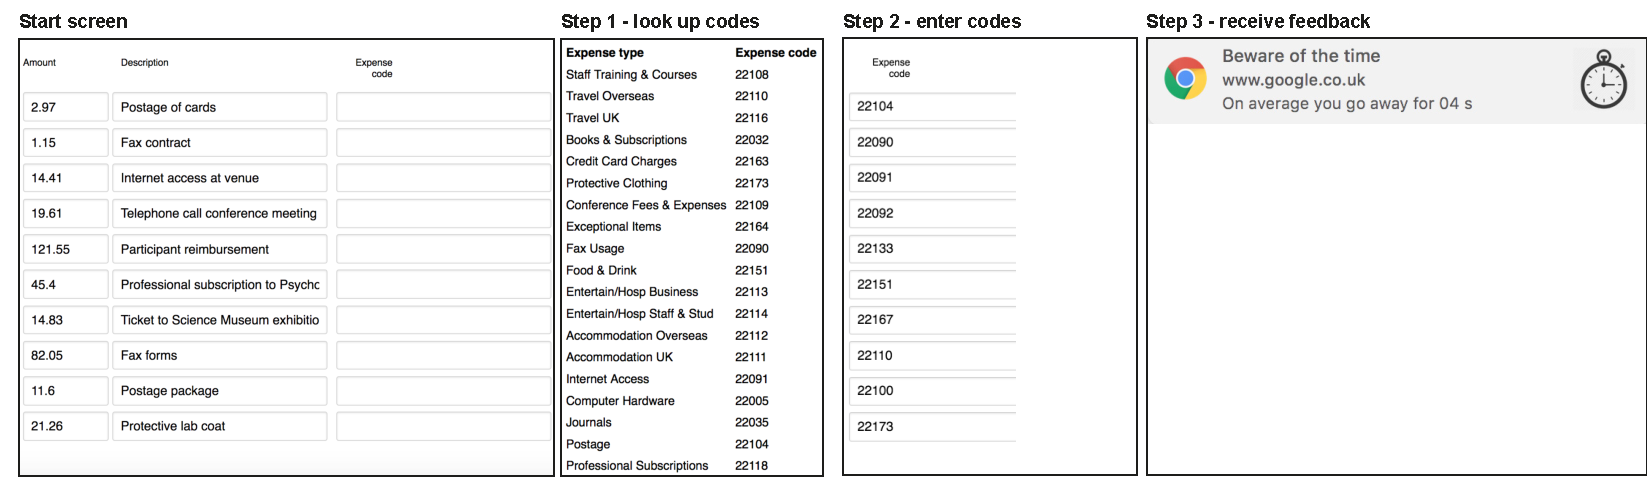
\includegraphics[width=\textwidth]{images/ch56/ch56-6_taskinterface.pdf}
\caption[Study 6 data entry task layout]{The data entry task as shown in the browser. Participants had to look up codes from their email (Step 1) and enter this into a sheet (Step 2). After every trial, the notification condition received time information (Step 3)}
%\vspace{-3pt}
\label{fig:ch56-6_TaskInterface}
\end{figure}

\subsubsection{Procedure}
The study was advertised online with a brief description and a website link to sign up. Participants signed up for the experiment by entering their email address, and were sent an email with the table of expense categories and expense codes. The email also included instructions with a new link where the study was available. Participants were asked to complete the task on a desktop or laptop computer and open the experiment in Google Chrome, Firefox or Safari. Participants were not informed beforehand which condition they had been allocated to, and were told the purpose of the study was to understand how people perform data entry tasks. Participants in the notification condition were informed that they would receive notifications during the experiment. 

Participants first read an online consent form on the website, and were not able to continue to the experiment until they had given explicit consent to participate. Participants in the notification condition received an additional dialog box to enable notifications in their browser, and had to click 'OK' to continue. Participants were instructed to have both their email and data entry window open on the same device, and to keep both windows maximised at all time, to ensure they had to switch back and forth between the two windows. 

After completing all experimental trials, participants were shown a page of debriefing information, explaining the purpose of the study. An email address was included as a point of contact if participants had any further questions. Participants took between 10 and 20 minutes to complete the experiment.

\subsubsection{Pilot study}
A pilot study was conducted with four colleagues to test the study set-up. Initially, the notification was set to appear on every switch, and showed the duration of the last interruption, instead of the average interruption time. Participant 1 looked at the notification at the start of the study, but experienced that the notification interfered with information she was holding in working memory. Upon switching, she had to memorise what expense category code she had to look up in the email, and looking at the notification made her forget what she was looking for, forcing her to go back to the data entry interface to look it up again. She therefore tried to ignore the notification for the rest of the study. For the remaining three pilot studies, the notification was adapted to only appear once after every trial, and show the average interruption duration. Two participants piloted the notification condition, and one participant piloted the control condition. Participant 3 used the information from the notification to try and find the codes in the email quicker, and consulted the notification after every trial to see whether his switches were shorter than the previous trials. The expenses task was experienced by participants as a realistic task, and all participants glanced at new incoming emails during the study.

\subsection{Results}
Table \ref{tbl:ch56-Table1} summarises the results of the conditions in terms of the four dependent variables. The number of switches, length of switches and the error rate were not normally distributed, so non-parametric Mann-Whitney tests were used to analyse effects of a notification on these dependent variables. A Shapiro-Wilk test suggested that the trial completion times were normally distributed, \textit{W} = 0.97, \textit{p} = 0.22, so an independent t-test was used to analyse the effect on trial times. A p-value of 0.05 was used for assessing the significance of all statistical tests. 

\begin{table}
\caption[Study 6 means and SDs of dependent measures]{Means and standard deviations of dependent variables for each condition.}
\centering
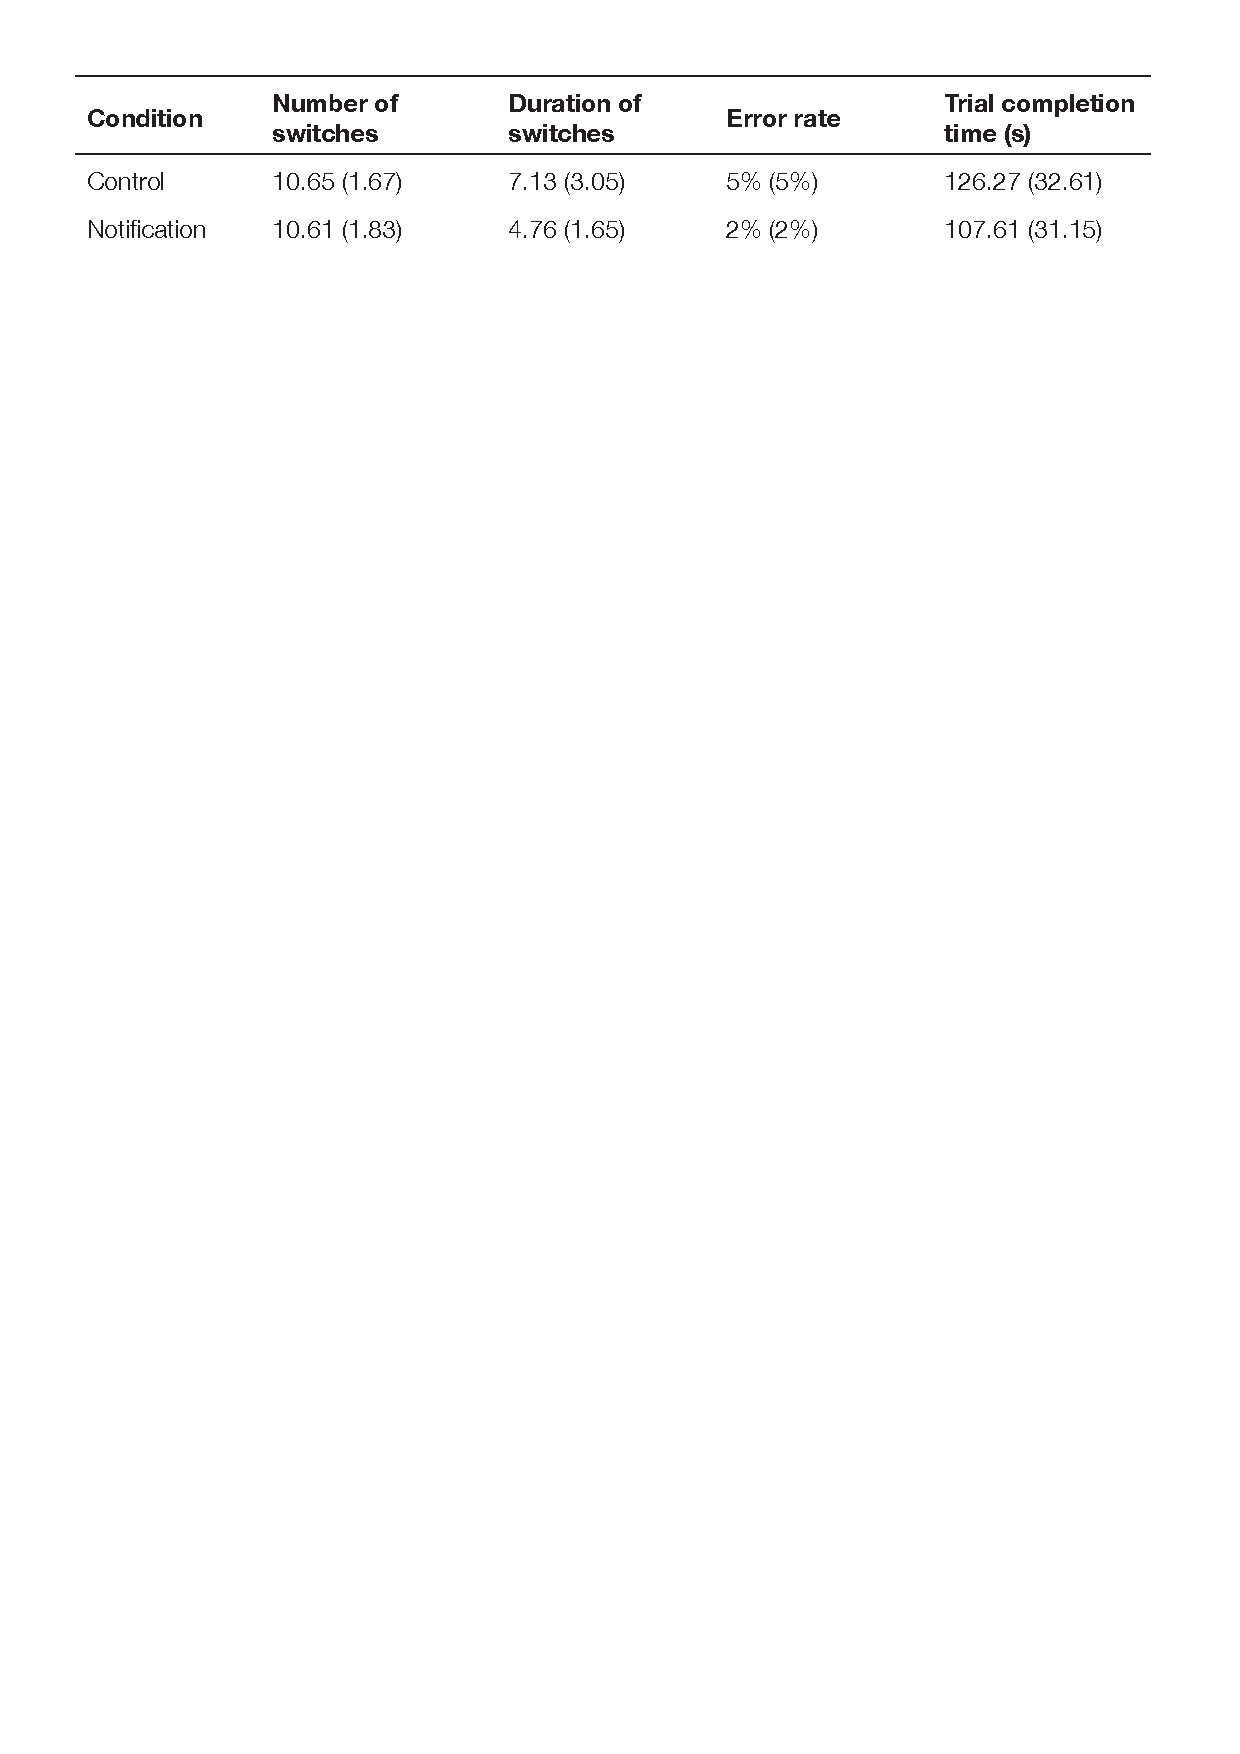
\includegraphics[width=0.9\textwidth]{images/ch56/ch56-descstats.pdf}
\vspace{-3pt}
\label{tbl:ch56-Table1}
\end{table}

\subsubsection{Cleaning the data}
In total, 87 participants signed up for the study. Thirty-four participants did not complete the task and their data was excluded from the dataset.
Furthermore, six participants made no recorded switches and were excluded from the dataset as well. Data from the remaining 47 participants was used in the data analysis.

\subsubsection{Task performance}
Participants with a notification were faster in completing trials (\textit{M} = 107.61s, \textit{SD} = 31.15s) compared to participants without a notification (\textit{M} = 126.27s, \textit{SD} = 32.61), \textit{t}(45) = 1.98, \textit{p} < .05, \textit{d} = .59.
Error rates were calculated by dividing the number of data entry errors divided by error opportunities. The error rates were significantly lower for participants with a notification (\textit{M }= 2\%, \textit{SD} = 2\%) compared to participants who had no notification (\textit{M} = 5\%, \textit{SD }= 5\%), \textit{U}(24, 23) = 403, \textit{p} < .01, \textit{r} = .44. 

\subsubsection{Number and duration of switches}
As can be seen in Table \ref{tbl:ch56-Table1}, participants who received notifications made significantly shorter switches (\textit{M}=4.76s, \textit{SD}=1.65s) than those in the control condition (\textit{M}=7.13s, \textit{SD}=3.05), \textit{U}(24, 23) = 406, \textit{p} < .01, \textit{r} =.44. The number of switches per trial was on average 10.6 in both conditions, and there was no significant difference in number of switches between conditions, \textit{U}(24,23)=243, \textit{p} = .60. As there were ten codes to be entered per trial, this suggests participants switched once for every piece of data entered. 

Figure \ref{fig:ch56-histswitches} shows the distribution of switching durations for the Control and Notification condition, the red line marks the mean duration. For both conditions, the distribution was positively skewed with a long tail: 97\% of the switches were under 20 seconds, but the longest switch was greater than seven minutes. To scale the distribution in one histogram, switches longer than 20 seconds are grouped as one bar. Table \ref{tbl:ch56-tblswitches} shows the count of these long switches for each condition, and highlights that there were some occurrences of very long switches, where participants were likely distracted. 

\begin{figure}
\centering
\begin{subfigure}{0.5\textwidth}
\centerline{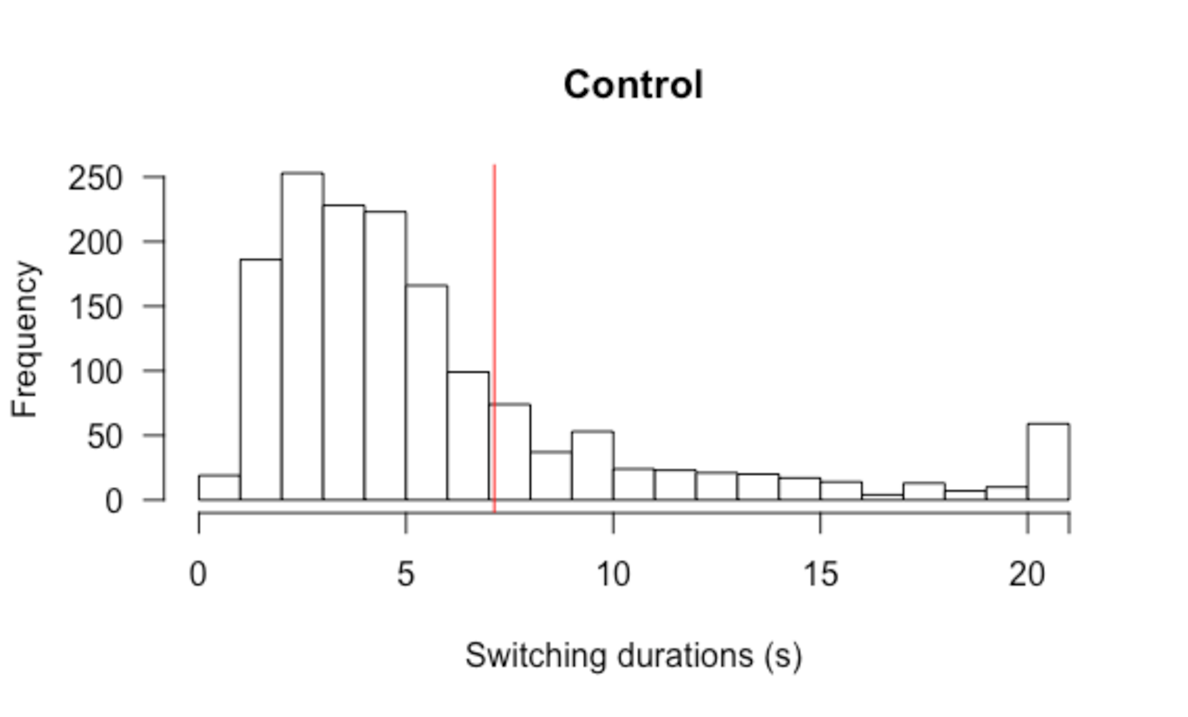
\includegraphics[scale=0.5]{images/ch56/ch56-histdurSwitches_Control.pdf}}
\end{subfigure}
\begin{subfigure}{0.5\textwidth}
\centerline{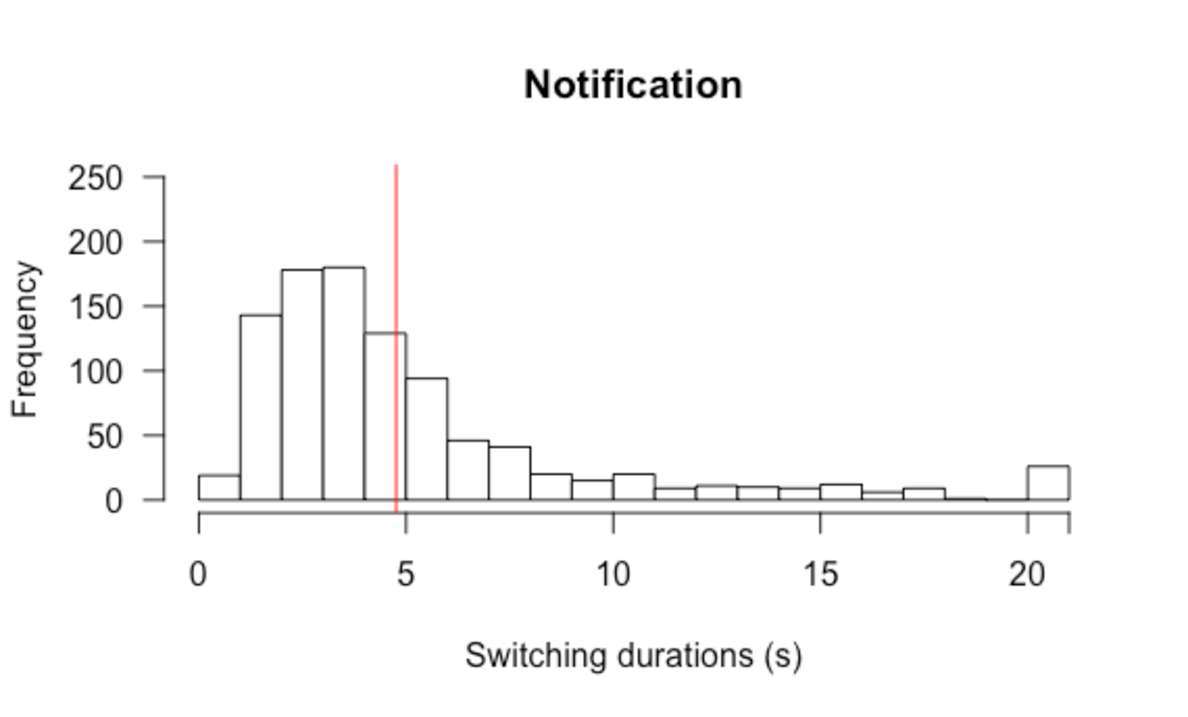
\includegraphics[scale=0.5]{images/ch56/ch56-histdurSwitches_Not.pdf}}
\end{subfigure}
%\vspace{-3pt}
\caption[Study 6 distribution of switching durations]{Histograms showing the distribution of switching durations for the two conditions; switches longer than 20 seconds are grouped in one bar at the right side of the histograms. The red line marks the mean switching duration.}
\label{fig:ch56-histswitches}
\end{figure}

\begin{table}
\centering
\centerline{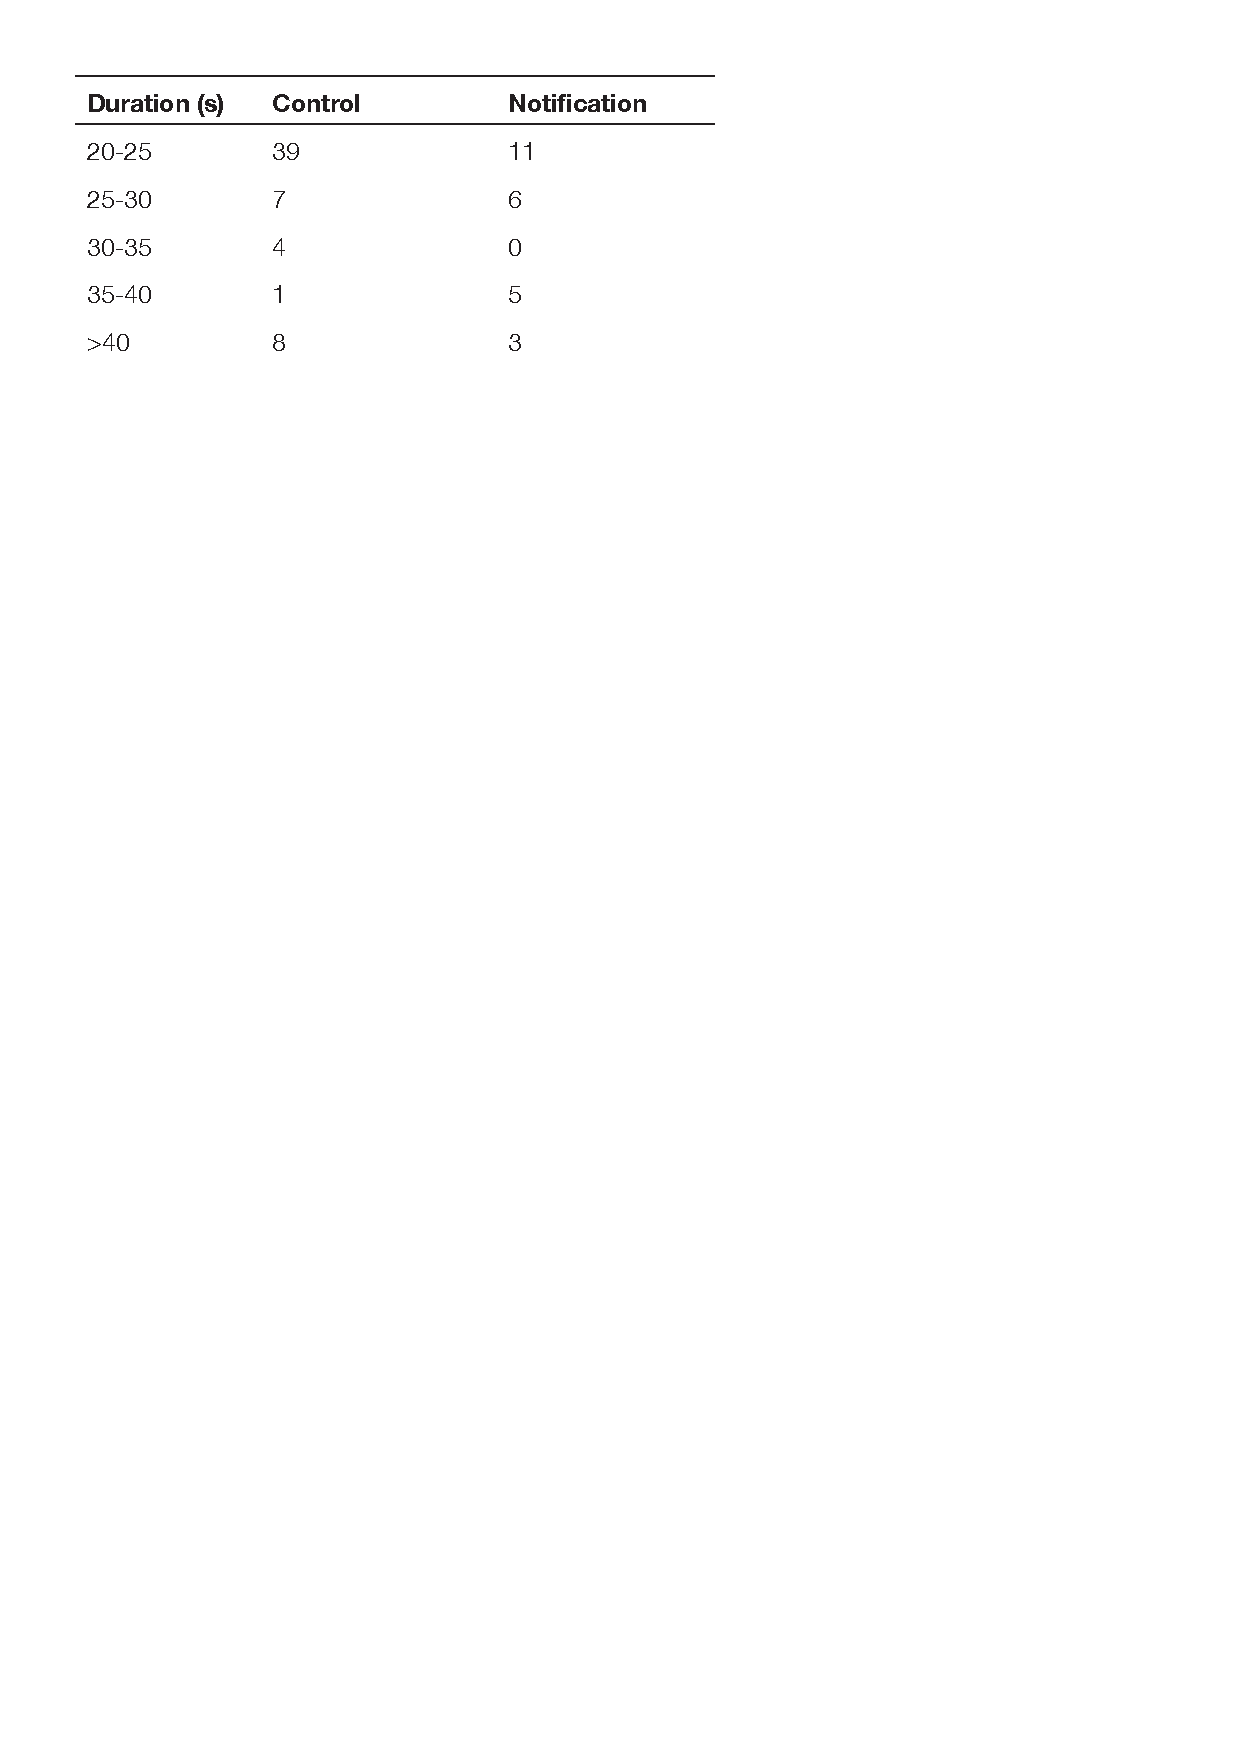
\includegraphics[scale=0.8]{images/ch56/ch56_LongSwitches.pdf}}
\caption[Study 6 frequency of long switches]{Total number of switches longer than 20 seconds for each condition.}
\label{tbl:ch56-tblswitches}
\end{table}

\subsubsection{Interkey intervals}
The primary measure to analyse switching behaviour were focus and blur events. These measures include any switch from the task window to another computer window. While this provides a good measure of digital switching behaviour, it cannot capture task switches outside the device because the task window remains in focus during these task switches (e.g., a user might pause to fetch a paper document or make a cup of coffee). To help capture this broader range of instances of possible task switching behaviour, I analysed longer pauses in task activity captured by an analysis of inter-keystroke interval (IKI) data. Though these intervals may have also been moments where participants had briefly paused for thought, extremely long intervals between two keystrokes may point to moments where a participant switched to doing something else. The IKI data presented here excludes intervals where a window switch was recorded, as these moments have already been analysed in the previous section.

There was no significant difference in duration of IKIs between the Control (\textit{M} = 1.70s, \textit{SD} = 0.91s) and Notification (\textit{M} = 2.02s, \textit{SD} = 1.60s), \textit{U}(24, 23) = 261.5, \textit{p} = .90. The mean IKIs are considerably longer than number typing speeds found in prior studies, which ranged from 180ms to 500ms \citep{Gould2016a}. The higher mean IKIs can be explained by looking at the whole distribution of all IKIs, as shown in Figure \ref{fig:ch56-histikis}. As can be seen from these histograms, the distribution was very skewed with a long tail which affected the mean IKIs. When considering the median rather than the mean, the median IKI was 192 ms in the Control condition and 305 ms in the Notification condition, which is more similar to a typical typing speed. Figure \ref{fig:ch56-histikis} shows that the majority of IKIs were under one second. There were however some instances when there were long delays between keypresses: the longest measured IKI is four minutes. In the histograms, IKIs longer than five seconds are grouped in one bar. To give a closer view of longer IKIs, Table \ref{tbl:ch56-tblikis}  shows the frequencies of long IKIs. These long IKIs were more than two deviations from the mean, and may have been additional task switches. However, we do not know for certain what people were doing during these instances, and what an appropriate IKI threshold would be to safely assume people had made a task switch. Therefore, we mainly focus our conclusions on our analysis of explicit window switches, and merely present the long IKIs to indicate that in addition to window switches, there may have been additional moments where people switched tasks. 

\begin{figure}
\centering
\begin{subfigure}{0.5\textwidth}
\centerline{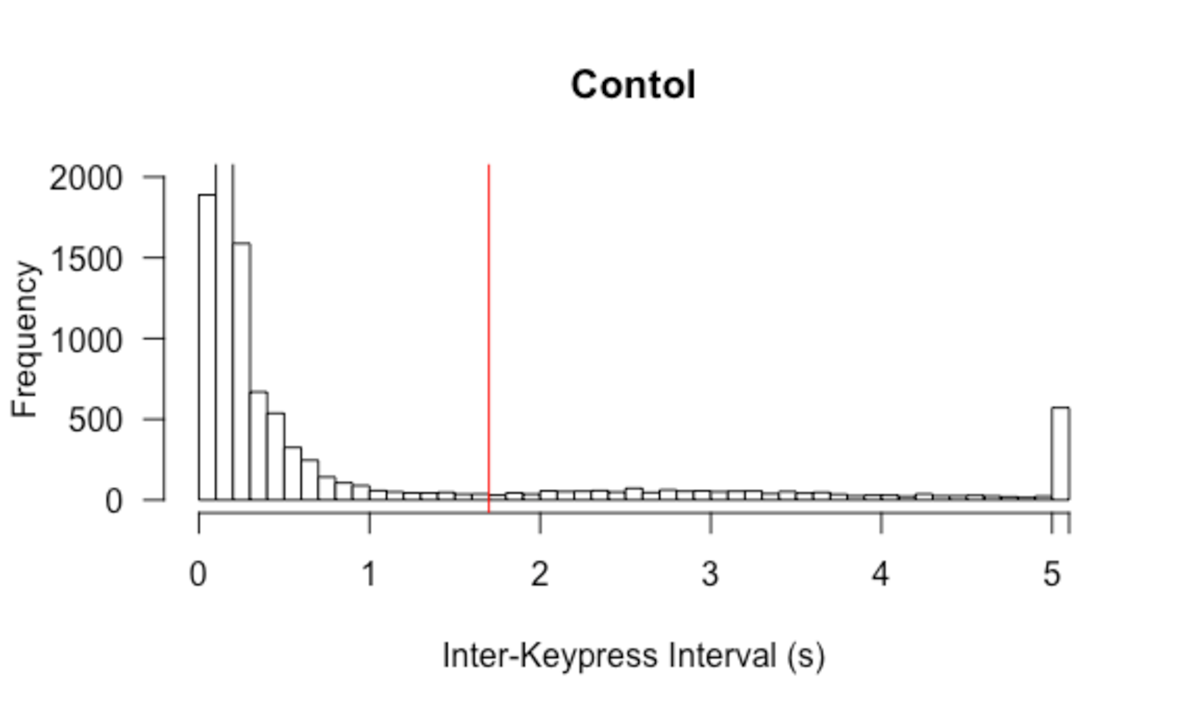
\includegraphics[scale=0.6]{images/ch56/ch56-histIKIs_Control.pdf}}
\end{subfigure}
\begin{subfigure}{0.5\textwidth}
\centerline{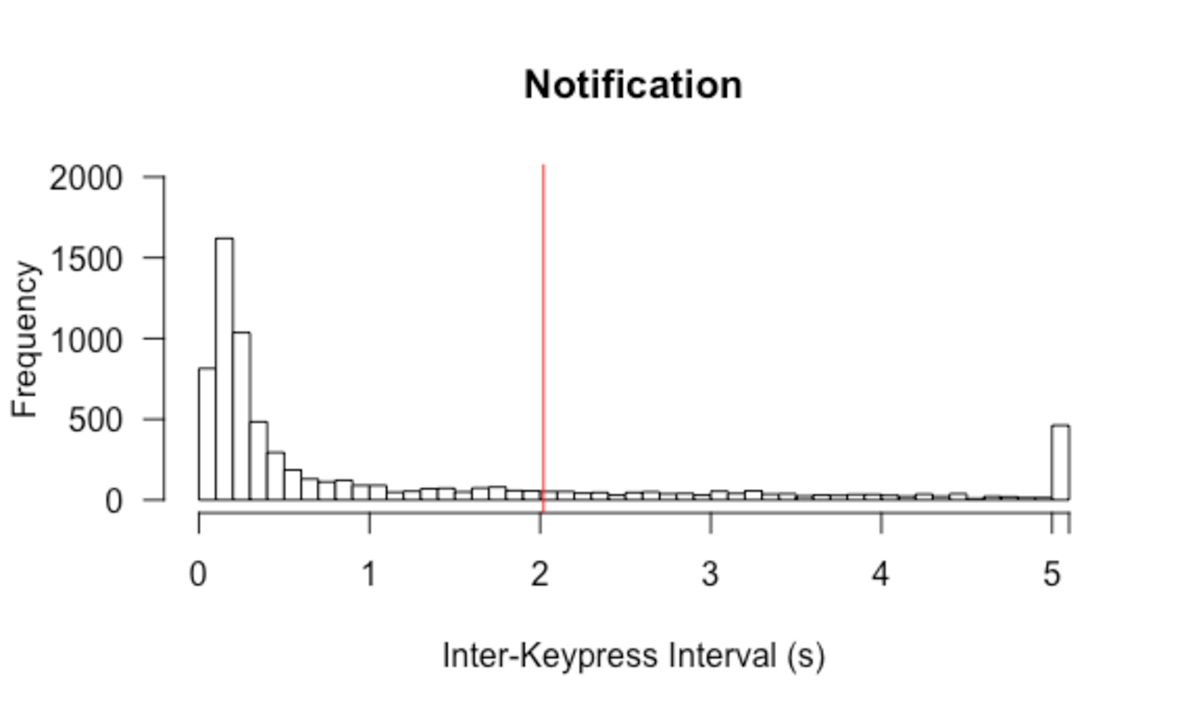
\includegraphics[scale=0.5]{images/ch56/ch56-histIKIs_Not.pdf}}
\end{subfigure}
\caption[Study 6 distribution of IKIs]{Histograms showing the distribution of inter-keypress intervals (IKIs) for the two conditions; switches longer than five seconds are grouped in one bar at the right side of the histograms. The red line marks the mean IKI.}
\label{fig:ch56-histikis}
\end{figure}

\begin{table}
\centering
\centerline{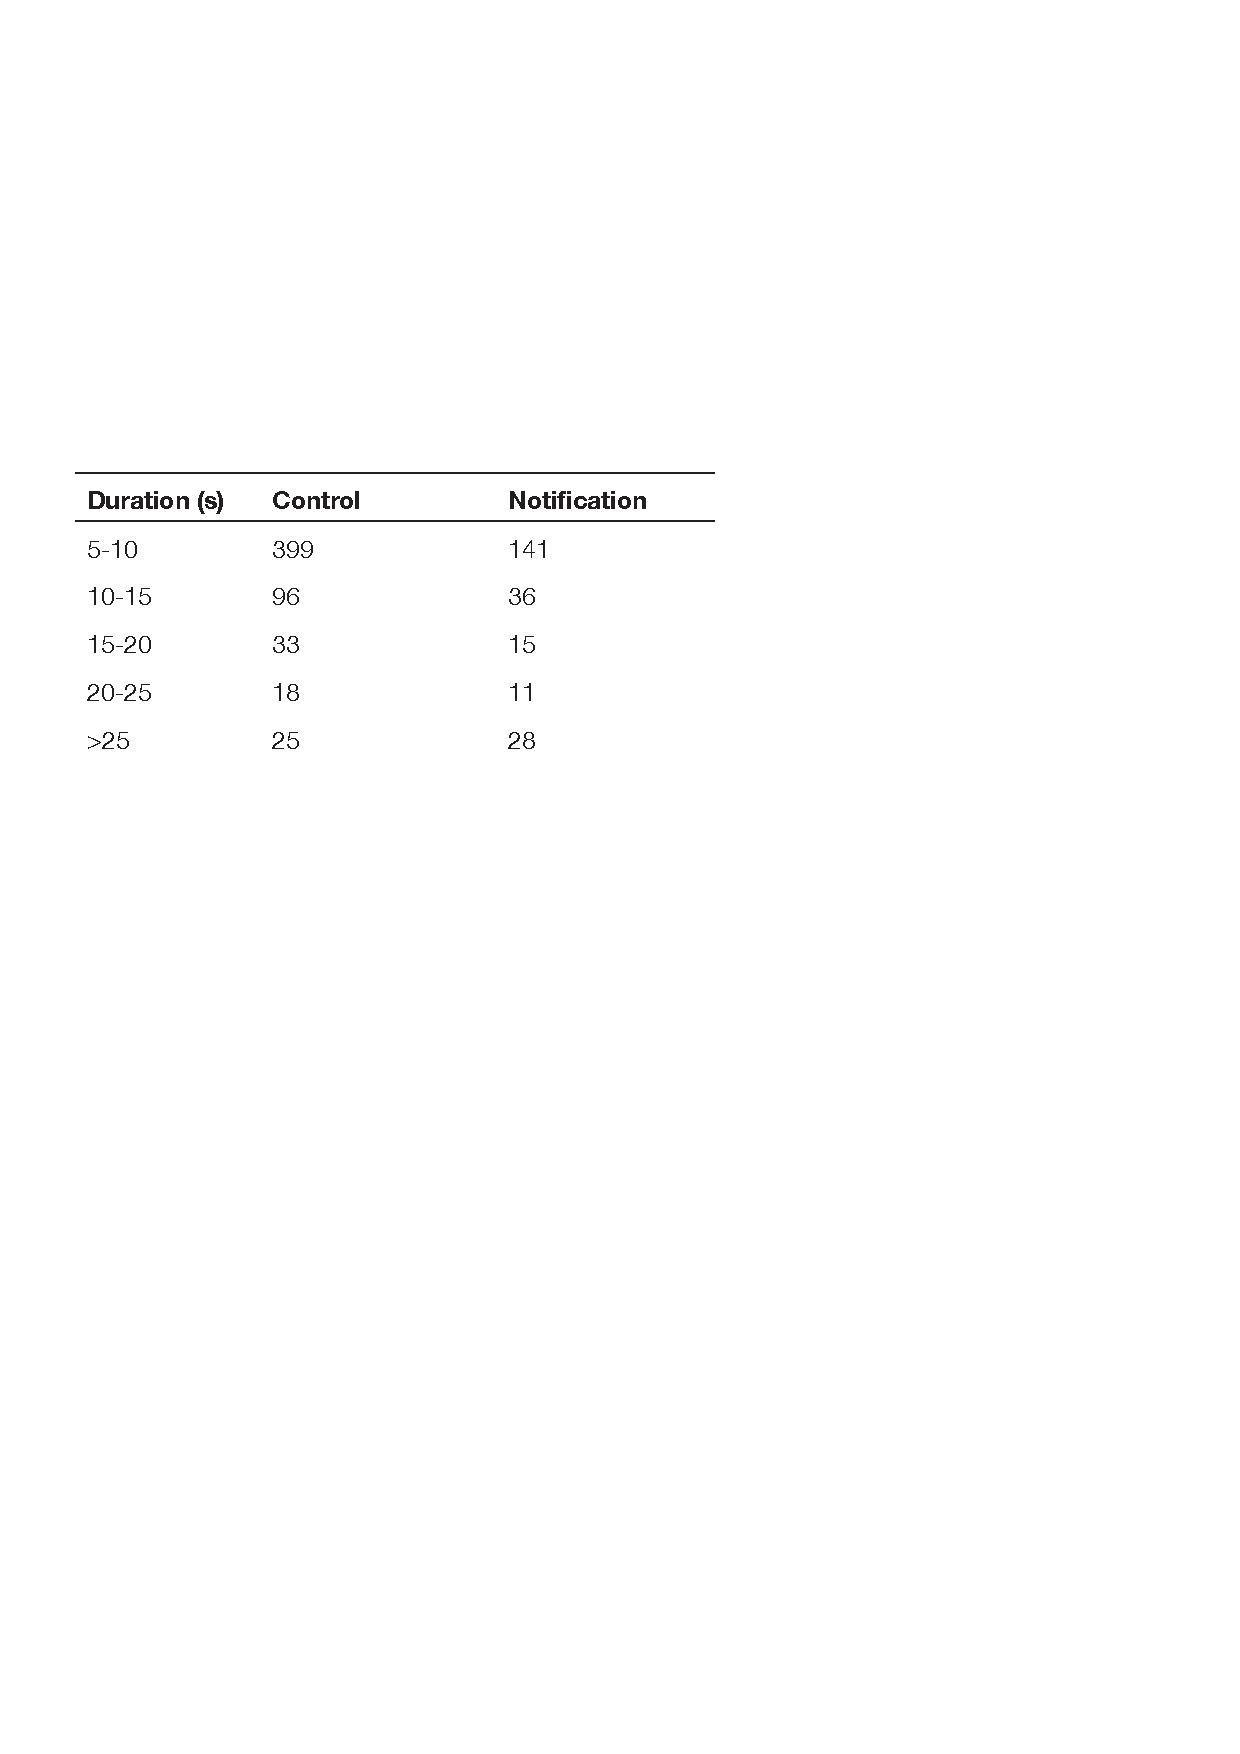
\includegraphics[scale=0.8]{images/ch56/ch56_LongIKIs.pdf}}
\caption[Study 6 frequency of long IKIs]{Total number of IKIs longer than 5 seconds for each condition.}
\label{tbl:ch56-tblikis}
\end{table}

\subsubsection{Effect of interruption duration on task completion time}
Participants who made longer switches took longer to complete trials. To see whether long switches also made people slower to resume a trial, we also consider trial completion times where the time spent on switches has been subtracted. For example, if a trial took 100 seconds, but the participant spent 20 seconds outside the task window, the adjusted trial completion time is 80 seconds.

With the adjusted trial times that has switching durations subtracted, I built a regression model to see if there was a potential relationship between trial completion times and number and duration of switches, as well as number and duration of IKIs. The linear model explained a significant amount of variation in trial times, ($R^2$ = 0.41, \textit{F}(5, 41) =5.68, \textit{p} < .01). Table \ref{tbl:ch56-linregr} shows there were three predictors that explained the variation: the number and duration of switches, and the number of IKIs. 

This model provides further insight into the effect of longer switches on task performance: the longer people switched for, the slower they were to finish a trial, even when switching durations are subtracted from the total trial time. The number of switches explained a smaller portion of the variation, but still had a significant effect. Furthermore, the more people typed, the slower they were to complete a trial.

\begin{table}
\centering
\centerline{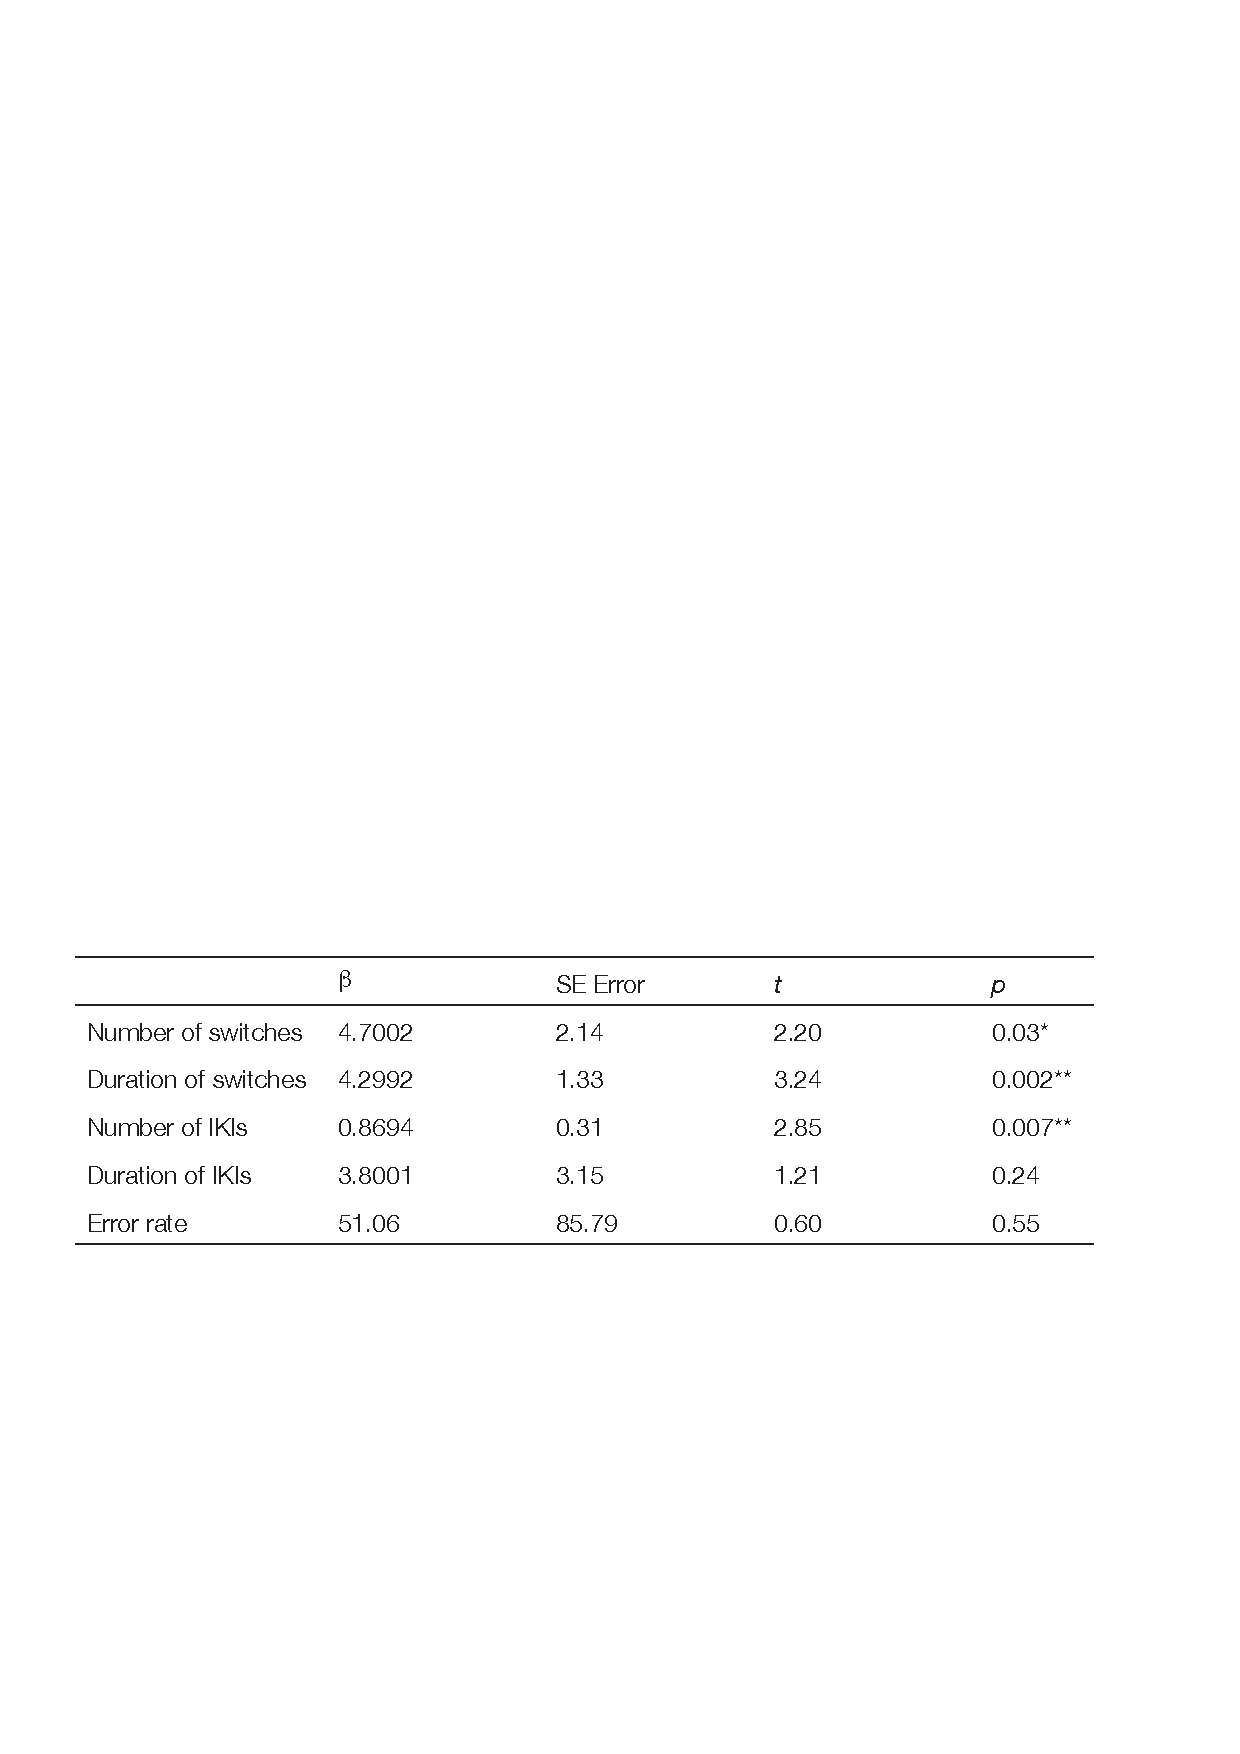
\includegraphics[scale=0.8]{images/ch56/ch56-linregr.pdf}}
\caption[Study 6 regression model to predict task completion time]{Predictors of regression model that predicts task completion time. An asterisk (*) indicates a predictor is significant at p < 0.05; a double asterisk (**) indicates a significance at p <0.01 level.}
\label{tbl:ch56-linregr}
\end{table}

\subsection{Discussion}
The aim of this study was to see whether showing people time feedback on how long they switched away from a task on average reduced the number and length of their inquiries. The results show that participants made shorter switches, were faster to complete the task, and made fewer errors. These results are important, as shortening interruptions may provide substantial benefits in work: it can make people less distracted and more concentrated on their current task, which can lead to higher productivity \citep{Iqbal2010, Mark2018}. The improvements in data entry accuracy and task completion time are also in line with previous experimental studies showing shorter interruptions improve task performance \citep{Altmann2017, Monk2008}. In these experimental studies, the length of the interruptions was controlled by the experimenters. The current study contributes to this body of work by exploring ways to shorten self-interruptions, where the length of the interruptions is controlled by users themselves.

Long switches significantly increased task completion time, even after subtracting the switching times. This can be explained by the resumption lag \citep{Altmann2004}: the longer people are away from a task, the longer it takes them to resume the primary task, as it takes longer to remember where people were in a task.
In addition to window switches, there were also some long pauses between keypresses, which suggests that people further self-interrupted themselves outside of the computer, with the task window still in focus. However, it is difficult to know for certain what was happening during these moments in a remote study. Without an accurate estimate of how long participants should take to complete the task, it is difficult to determine moments at which participants were away from their computer \citep{Rzeszotarski2013}. Future studies could use additional metrics to explore what people are doing during long pauses: for example, the data entry interface may prompt the user to confirm they are still working on the task, after a certain amount of inactivity.

Most experimental studies on self-interruptions have used an artificial distraction, such as chat messages, to measure how people self-interrupt to attend to this distracting task \citep{Katidioti2013, Salvucci2010}. The current study makes a methodological contribution by using participants' own personal email inbox, based on the assumption that email provides a natural source of distraction \citep{Hanrahan2015, Mark2016}. The benefit of using an experimental task is that it enabled me to log data entries and measure a direct effect on task performance. 
In the current study, participants only needed to find and open an email once. Once they had this email opened, they did not have to re-find it in their inbox for the remainder of the experiment, and may have had this email maximised on their screen, hiding incoming messages. In practice however, people have to first find the email in their inbox, which can partly contribute to the distraction. This study has already shown an effect on behaviour by switching to an email inbox. It is expected there might be a higher potential for distraction if people have to also find the correct email in their inbox.

Giving participants feedback on the duration of their switches did not reduce the overall occurrence of switches as in prior work \citep{Gould2016a}. A reason for this difference in results may be that in prior work, feedback was given after every switch, whereas in this study feedback was only given after every trial. As participants had to switch regularly as part of the task, giving notifications at every switch would have had the risk of overexposing participants to notifications and limiting its usefulness \citep{Cutrell2001, Whittaker2016}. When piloting the study, a notification after every switch was found to be too disruptive, and interfered with memorising what people were interrupting themselves for. Therefore, feedback was only given after every trial. A future study could explore showing people the number of times they switch away from a task, in addition to the duration of switches. As people work to maximise their task performance based on the explicit feedback that they are given \citep{Farmer2017}, showing people the number of switches away from a task may encourage them to reduce the number of switches.

\subsubsection{Conclusion}
The results of this experiment indicate that showing people how long they switch on average reduces the duration of switches and can improve people's task performance. The work makes a contribution to our understanding of switching behaviour for routine data entry tasks to distracting, but task-relevant, applications such as email. The results also suggest ways in which tendencies to attend to distractions might be mitigated, and can provide a useful pointer for the design of productivity interventions to improve focus.

One of the factors that influence the costs of a work interruption is its length: while short interruptions can be beneficial to productivity, too many interruptions and for too long take valuable time away from work \citep{Mark2018}. Based on this, together with the finding that time feedback reduces the duration of interruptions, it is expected that time feedback can make people more focused and productive in their work.  In the current study, an experimental task was used in order to measure task performance. The focus of the study was on the effect of time feedback on duration of interruptions, and did not explore people's underlying motivations for their behaviour, and whether people indeed felt more focused or productive. Perhaps people were motivated to be focused on the task as they knew it was part of an experiment.

To investigate whether the effects of time feedback generalise beyond an experiment and are of real benefit to people working in office settings, Study 7 tested the notification with office workers doing their own data entry work.They were asked to install and use the notification on their work computer for two weeks, and were interviewed afterwards on their experience of using the tool.

%The study did not find any effect on the number of switches. However, as the number of switches indicate, participants presumably only switched to look up information, and did not switch to other tasks, interruptions or distractions. When people are doing their own data entry work, they may not have to switch as often as in the current experiment, but on the other hand they may interrupt themselves more to attend to other tasks and interruptions. To evaluate whether the positive effect of time feedback on people's switching behaviour can extend to naturalistic tasks, Study 7 tested the notification with office workers doing their own data entry work,

\section{Study 7: Looking up information for expenses in an office setting}\label{st:Study7}
\subsection{Introduction}
In order to understand whether showing people how long they go away from a task would have the same effect on a naturalistic data entry task, Study 6 was followed up with a field study testing the notification with data entry workers doing expenses work. To measure self-interruption behaviour during their work, participants were asked to install a free trial version of ManicTime \footnote{https://www.manictime.com} for two weeks. ManicTime is a time tracking software, which tracks application and web page usage. In addition, participants were asked to install a browser extension, and use it when they are processing expenses. Every time participants switched away from the browser window in which they did their expenses work, the extension showed a notification similar to the notification used in Study 6. The purpose of the study was to see whether a notification had an effect on self-interruption behaviour. To get a quantitative measure of self-interruption behaviour, ManicTime data was used to derive number and duration of window switches during expenses work. In addition, participants were interviewed to explore whether and how the use of both the extension and ManicTime led to any conscious changes in their behaviour. The study aimed to address the following question: how does time feedback on interruption length have an effect on people's self-interruption behaviour during expenses work in a finance office setting? 

\subsection{Method}
%DESIGN
To study the effect of a notification on people's self-interruption behaviour, I originally planned to use a between-groups design: participants would be divided into a control group and experimental group. The control group would be asked to install ManicTime for two weeks. They would be told the purpose of the study was to understand how people in offices manage tasks, windows and applications. The experimental group would also be asked to install ManicTime, but would additionally be asked in the second week to install the browser extension. They would be told that this extension would give additional information on the current task they were working on. Other than this distinction, all instructions would be identical between the two groups. However, upon conducting the study, five participants were unable to install ManicTime on their work computer due to security restrictions. Therefore, there was insufficient quantitative data collected to make a comparison in switching behaviour between conditions. Instead, the study's focus became the qualitative data collected during the interviews, and all participants used the browser extension in the second week. Participants who were able to install ManicTime did so at the start of the first week and kept it running for two weeks. In the second week, all participants were asked to install the browser extension.
%Four participants were unable to use Google Chrome, and therefore the extension, for their work. Therefore, these participants were part of the control group. To make the groups even, one other participant was randomly chosen to be allocated to the control group; the remaining participants were allocated to the experimental group. 

%If the main task page is not in focus, either because participants have switched to another page or if it has been inactive for x seconds, they will receive a notification with a warning message. Upon returning to the expenses page, they will receive a notification indicating how long they were away from the page. The control group will be asked to install the plug-in, but will receive no notifications. It is explained that the purpose of the study is to log people's switching behaviour, and participants will be able to see their data at the end of the study. Participants will be asked to use the add-in for one week in which they have to do a substantial amount of expenses work, and keep a diary of their experiences. Within a week of finishing the diary, a follow-up interview will be scheduled to gather more detailed explanations of participants' experiences of using the add-in.

\subsubsection{Participants}
Nine participants (six female) took part in the study. They were office workers at finance administration offices at one of the public universities from Chapter 3, and were invited to participate via emails sent to departmental mailing lists and snowballing. Participants worked in an open plan office, and seven participants occasionally worked from home. Participants’ work included administrative and supportive tasks, such as processing payments, expenses, managing budgets, and responding to queries by university staff and students. The majority of participants’ work was carried out in a web browser, and revolved around a number of web-based data entry systems. None of the participants had used a time or task management tool before. Participants were reimbursed with a  \pounds 20 Amazon voucher after completing the study. 

%Ten participants (three male) took part in the study. They were recruited using the same recruitment methods as Study 1 and 2. Invitations were sent to opt-in mailing lists of Finance departments of a university, and forwarded by contact persons and people who had already participated. None of the participants had taken part before in any of the studies reported in this thesis, but were drawn from the same population. None of the participants had used a time management application such as ManicTime before. Participants were reimbursed with a \pounds 20 Amazon voucher.

\subsubsection{Materials}
The notification was implemented as a Google Chrome extension using HTML, JavaScript and CSS. After installing the extension, an icon was permanently visible in participants’ browser (see Figure \ref{fig:ch56-7_taskinterface}). To use the extension, participants had to navigate to a web page in their web browser that they wanted to focus on, and click on the icon of the extension. Upon clicking on the icon, a pop-up appeared saying that the current web page was now the main task page, which indicated the start of a task session. Every time participants switched away during the session from this web page to another computer window, such as a different browser window, a document or an application, they received a notification indicating how long on average they go away for when switching away from the main task page. If participants switched away from a page for the first time, the notification showed a message that no switching data was available yet. To calculate the average switching duration, the extension recorded and saved the number and duration of switches away from the main task page for the whole session. Participants ended a session by closing the page. Due to security restrictions of browser extensions, the extension was unable to save any session data after a session had ended. 

\begin{figure}
\centering
\centerline{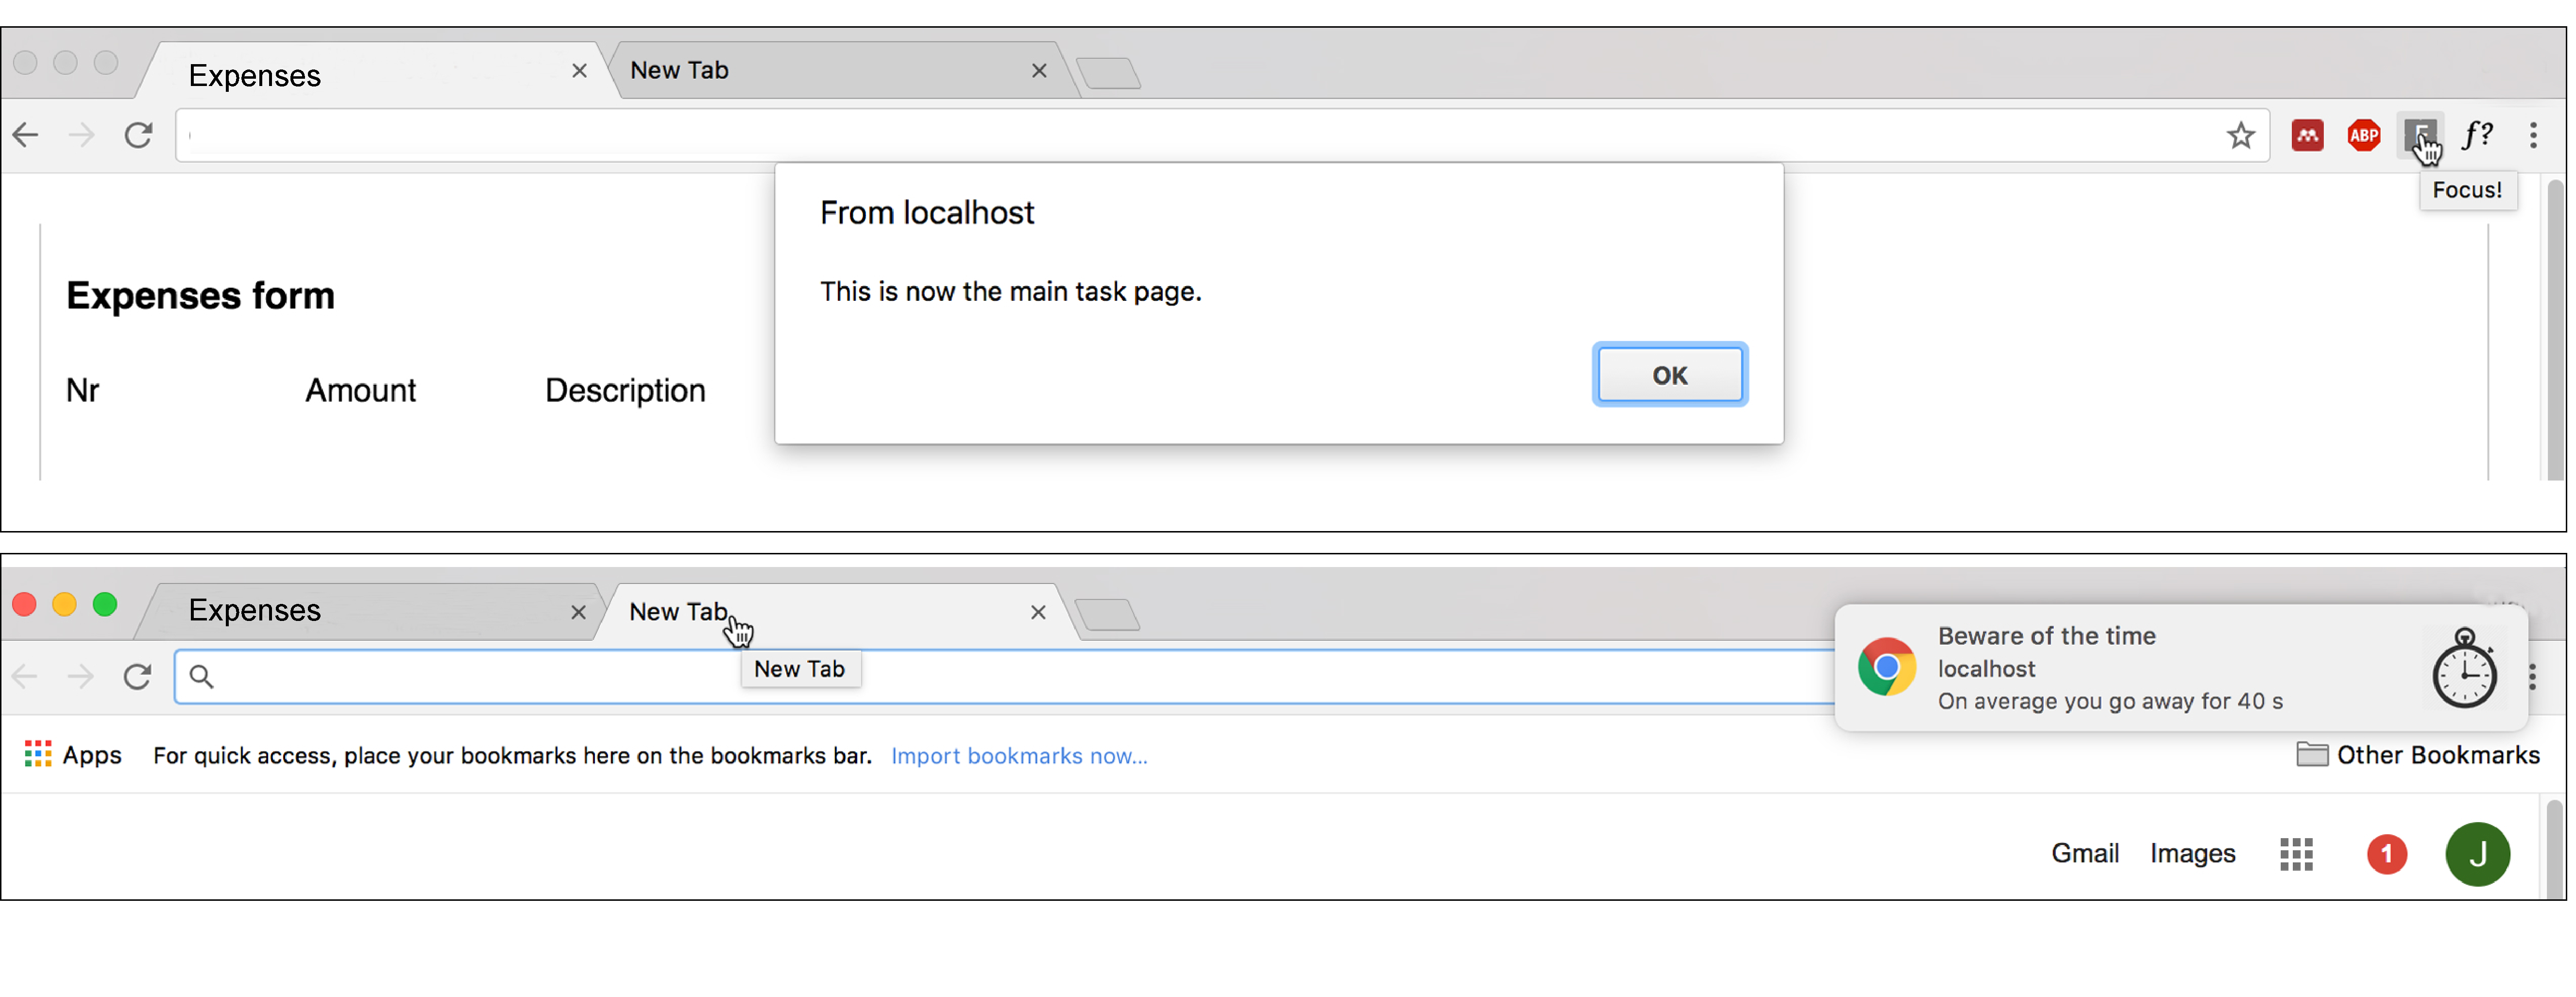
\includegraphics[scale=0.17]{images/ch56/ch56-7_taskinterface.pdf}}
\caption[Study 7 browser extension]{Participants selected a web page to focus on by clicking on the extension icon in their browser, after which a popup appeared to confirm this was now the main task page. Every time the participant switched to another window, application or document, a browser notification showed how long on average they switch away from this page.}
\label{fig:ch56-7_taskinterface}
\end{figure}

The presentation of the notification was similar to Study 6 but differed in one important aspect. Whereas the notification in Study 6 appeared once after every trial, in this study it appeared upon every switch away from the task. Based on the observations and interviews reported in Chapter 3, I anticipated participants switched less frequently for their main work compared with the experimental task, and therefore a notification at every switch was not considered to be too disruptive.

To get an understanding of people’s interruption and window switching behaviour, participants were also asked to install ManicTime, a computer logging software which records and stores the time spent in all application windows. I initially intended to give the extension to only half of the participants to see if there was a notable difference in interruption behaviour between people who used the extension compared to people who did not. However, five participants were unable to install ManicTime on their work computer, and could only use the extension. Due to this lack of quantitative data to make a fair comparison, I therefore distributed the extension to all participants and mainly focused on the interviews and people’s experience of using the tool. A summary of ManicTime data of the remaining four participants (P3, P4, P5 and P9) is included in this chapter and used to complement the qualitative interview data and give an insight in the fragmented nature of people’s work.

\subsubsection{Procedure}
Participants who expressed interest were sent an information sheet and consent form to read and sign. They were sent an overview of the study, instructions to install the tools, and a post-study interview was scheduled.
The study was divided into three stages:

\textit{Week 1: Install ManicTime}

In the first week, participants were sent instructions to install ManicTime on their work computer. They were given the option to pause or stop the application from running at any time. They were told that they were free to choose if, when and how often to look at the information, but that it was important to complete at least one expenses task with the application running. 

\textit{Week 2: Install the browser extension}

In the second week, participants were asked to install the extension. Again, they were instructed that they were free to choose when and how often to use the extension, but that they had to use it for at least one expenses task. %Even though the second week was the same for participants in the control condition, they were also asked to complete at least one expenses task in the first week, and another expenses task in the second week. This instruction was included to compare if any observed changes in switching behaviour were due to the browser extension, or if participants simply became more aware of their switching behaviour in the second week.

\textit{Week 3: Interview}

%Participants were sent an email with instructions on how to share their database and remove the tools from their computer.
After two weeks, participants were interviewed about how they currently manage documents, applications and tasks for their work, and asked questions on their experience of using the tools. In particular, it was discussed whether and how they used or would use the information that the tools provided, and whether they made any changes on how they went about their work. They were asked to share their ManicTime database for further analysis. Participants were offered guidance and assistance on deleting or adapting any data in their database, such as removing application and website names. Participants were still eligible to participate, if they did not wish to share their database.

The interviews were structured around the following themes: how participants currently manage interruptions, tasks, time and information, the context of using the extension, the usefulness of the information provided by the extension and ManicTime, and whether they made any changes on how they managed their work. Participants who did not install ManicTime were presented with screenshots during the interview, and discussed the usefulness of this type of information compared to the time information of the extension. An interview lasted about 60 minutes and was audio recorded. 

\subsubsection{Pilot study}
A pilot study was conducted with two participants. One participant was a colleague and was sent instructions to install the browser extension on his computer. The purpose of this pilot session was to see whether the installation instructions were clear and to test the extension on other people's computers. The participant had the tendency to hover over the notification to stop it from disappearing, which placed extra buttons over the end of the notification message. Therefore, the message was shortened and the most important information, namely the duration of switches, was placed at the front of the message to ensure it was still visible upon hovering.

A second pilot session was then conducted with an administrator working at the same university as the study participants, who was asked to install ManicTime and the extension on her work computer. The purpose of this session was to ensure the tools could be installed on the work computers of the university, and that the extension worked with the university finance system.

%Findings pilot study

\begin{comment}
\subsubsection{Ethical considerations}
Participants were informed before undertaking the study that they would be asked to share their ManicTime database at the end of the study. However, a disclaimer was added in the invitation and instruction emails that participants were still able to take part, if they did not wish to share their database. It was made clear what data ManicTime recorded, and that Focus did not store any data. They were given instructions on how to pause the application from running and how to delete certain parts of the data, and were offered assistance to help further change the database into a state they were comfortable sharing. 
\end{comment}

\subsubsection{Data analysis}
Though ManicTime was piloted on a work computer of the university before starting the study, five participants were unable to install ManicTime on their work computer due to firewall restrictions. It appeared that different participants had different computers, operating systems and firewall settings. %Furthermore, two participants opted out of using Focus as they used a browser different from Google Chrome for at least parts of their work. 
Therefore, ManicTime data of the remaining four participants was used to complement qualitative explanations of their task switching behaviour, but it was not analysed quantitatively as previously planned to compare switching behaviour with and without the extension. Instead, the primary focus of data analysis was on the post-study interviews and participants' subjective experience of using the tools. The interviews were transcribed verbatim, and analysed using thematic analysis.

\subsection{Findings}
%Reflective and current information
Participants gained some insights to change their behaviour based on the information they received from the extension. People’s switching behaviour as shown by the ManicTime data is reported first. I then discuss the usefulness of time feedback to manage interruptions around the following themes: awareness and change of behaviour, the type of interruptions, the effort to record and use data, setting goals, and the work environment.

\subsubsection{Switching behaviour}
Participants’ working hours differed slightly, but all participants worked at least ten hours per day during the study. To make the data comparable between participants, I only considered data between 9am and 7pm, during which all participants were at work. As I was only able to gather logging data from five participants, there is insufficient data to make a fair comparison between switching behaviour without and with the extension. Summary data is presented here to give insight into people's switching behaviour during the study, but these are not analysed using any statistical models.

Table \ref{tbl:ch56-7_manictimedata} summarises the average number and duration of focus on a computer window screen. The mean duration of focus is about 34 seconds, with the longest focus being 45 minutes (2733 seconds). On average, participants made 696  computer window switches per working day. Figure \ref{fig:ch56-7_histswitches} shows the distribution of all window focus durations, illustrating that participants were rarely focused on a window for more than a minute. To scale the histogram, window focus durations longer than 150 seconds are grouped in one bar; the frequency of these longer durations are shown in Table \ref{tbl:ch56-tblwindowdurations}. %The distribution of window focus durations was positively skewed with a long tail: 95\% of the distribution is plotted in Figure 8, illustrating that participants were rarely focused on a window for more than a minute. 
Together with the interview findings, the data shows that participants’ work was characterised by short durations of focus and frequent window switches. %Figure \ref{fig:ch56-7_mtdurswitches} and Figure \ref{fig:ch56-7_mtnrswitches} show the average number of daily window switches and focus durations over the ten days of the study.

In addition to computer window switches, participants also made a smaller number of non-digital interruptions, for example when taking a break or attending a meeting (see Table \ref{tbl:ch56-7_manictimedata}). On average participants made three daily non-digital interruptions which lasted about 29 minutes (1741 seconds). 

\begin{table}
\centering
\centerline{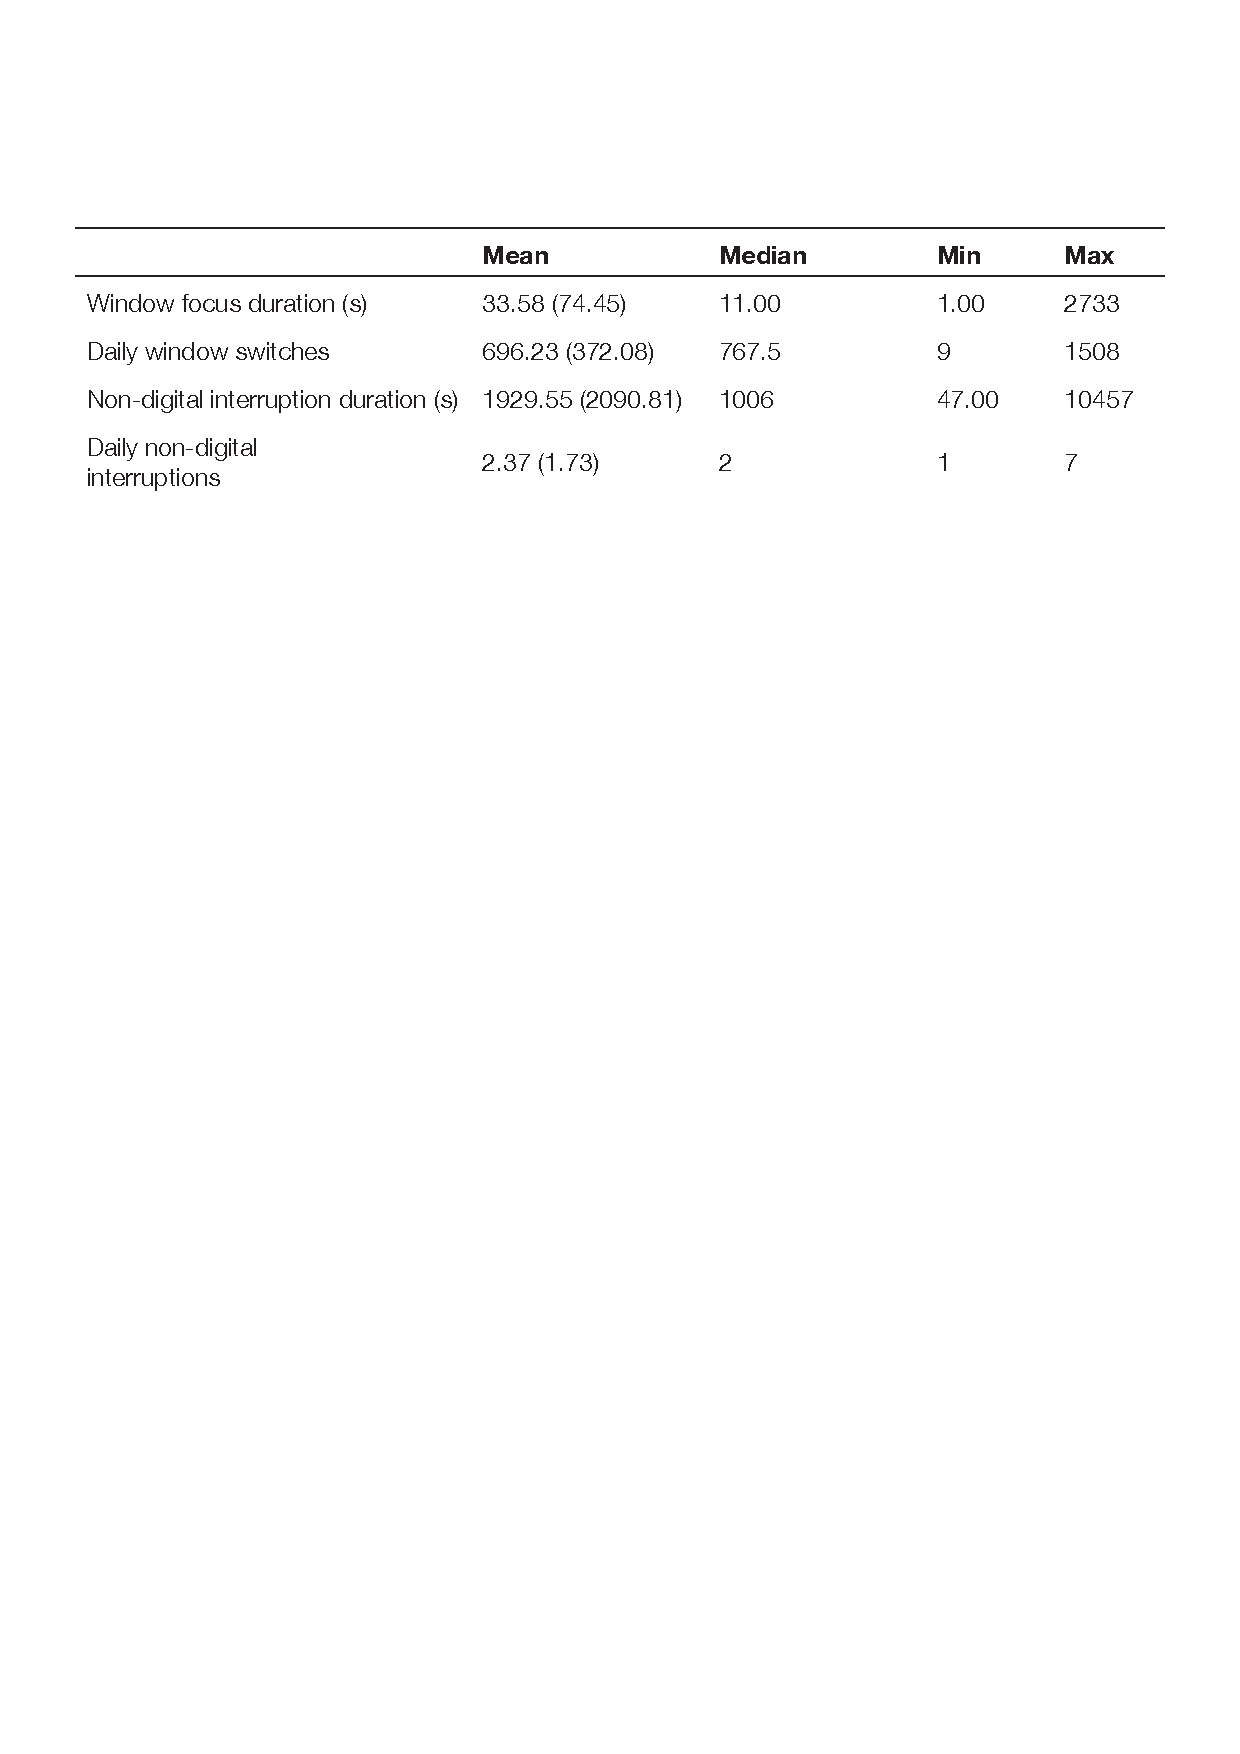
\includegraphics[scale=0.7]{images/ch56/ch56_7_Means.pdf}}
\caption[Study 7 window switching behaviour]{Average window focus durations (s) and number of daily switches.}
\label{tbl:ch56-7_manictimedata}
\end{table}

\begin{figure}
\centering
\centerline{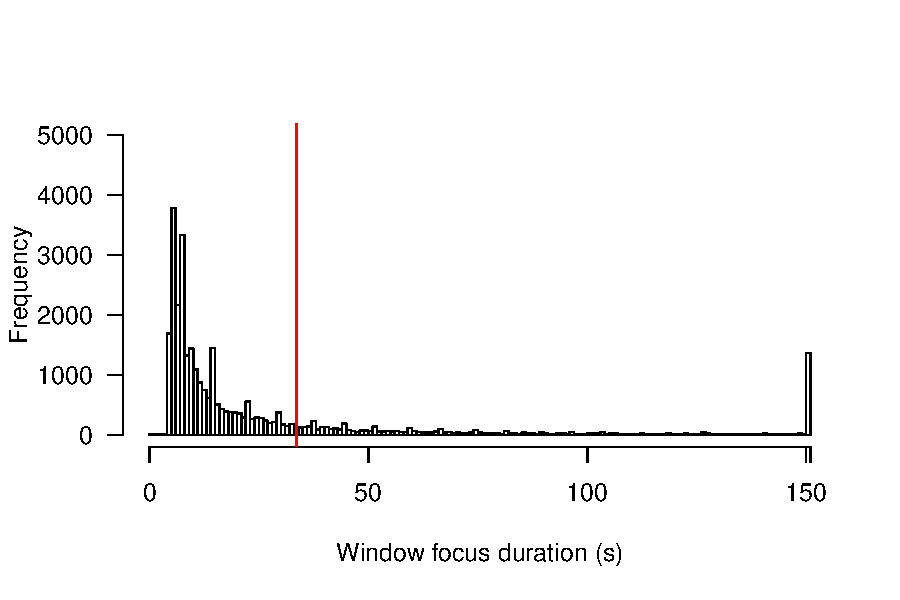
\includegraphics[scale=0.8]{images/ch56/ch56-7_WindowSwitches.pdf}}
\caption[Study 7 distribution of window focus durations]{The distribution of window focus durations during the study, measured by ManicTime. Durations longer than 150 seconds are grouped in one bar at the right side of the histogram. The red line marks the mean window focus duration.}
\label{fig:ch56-7_histswitches}
\end{figure}

\begin{table}
\centering
\centerline{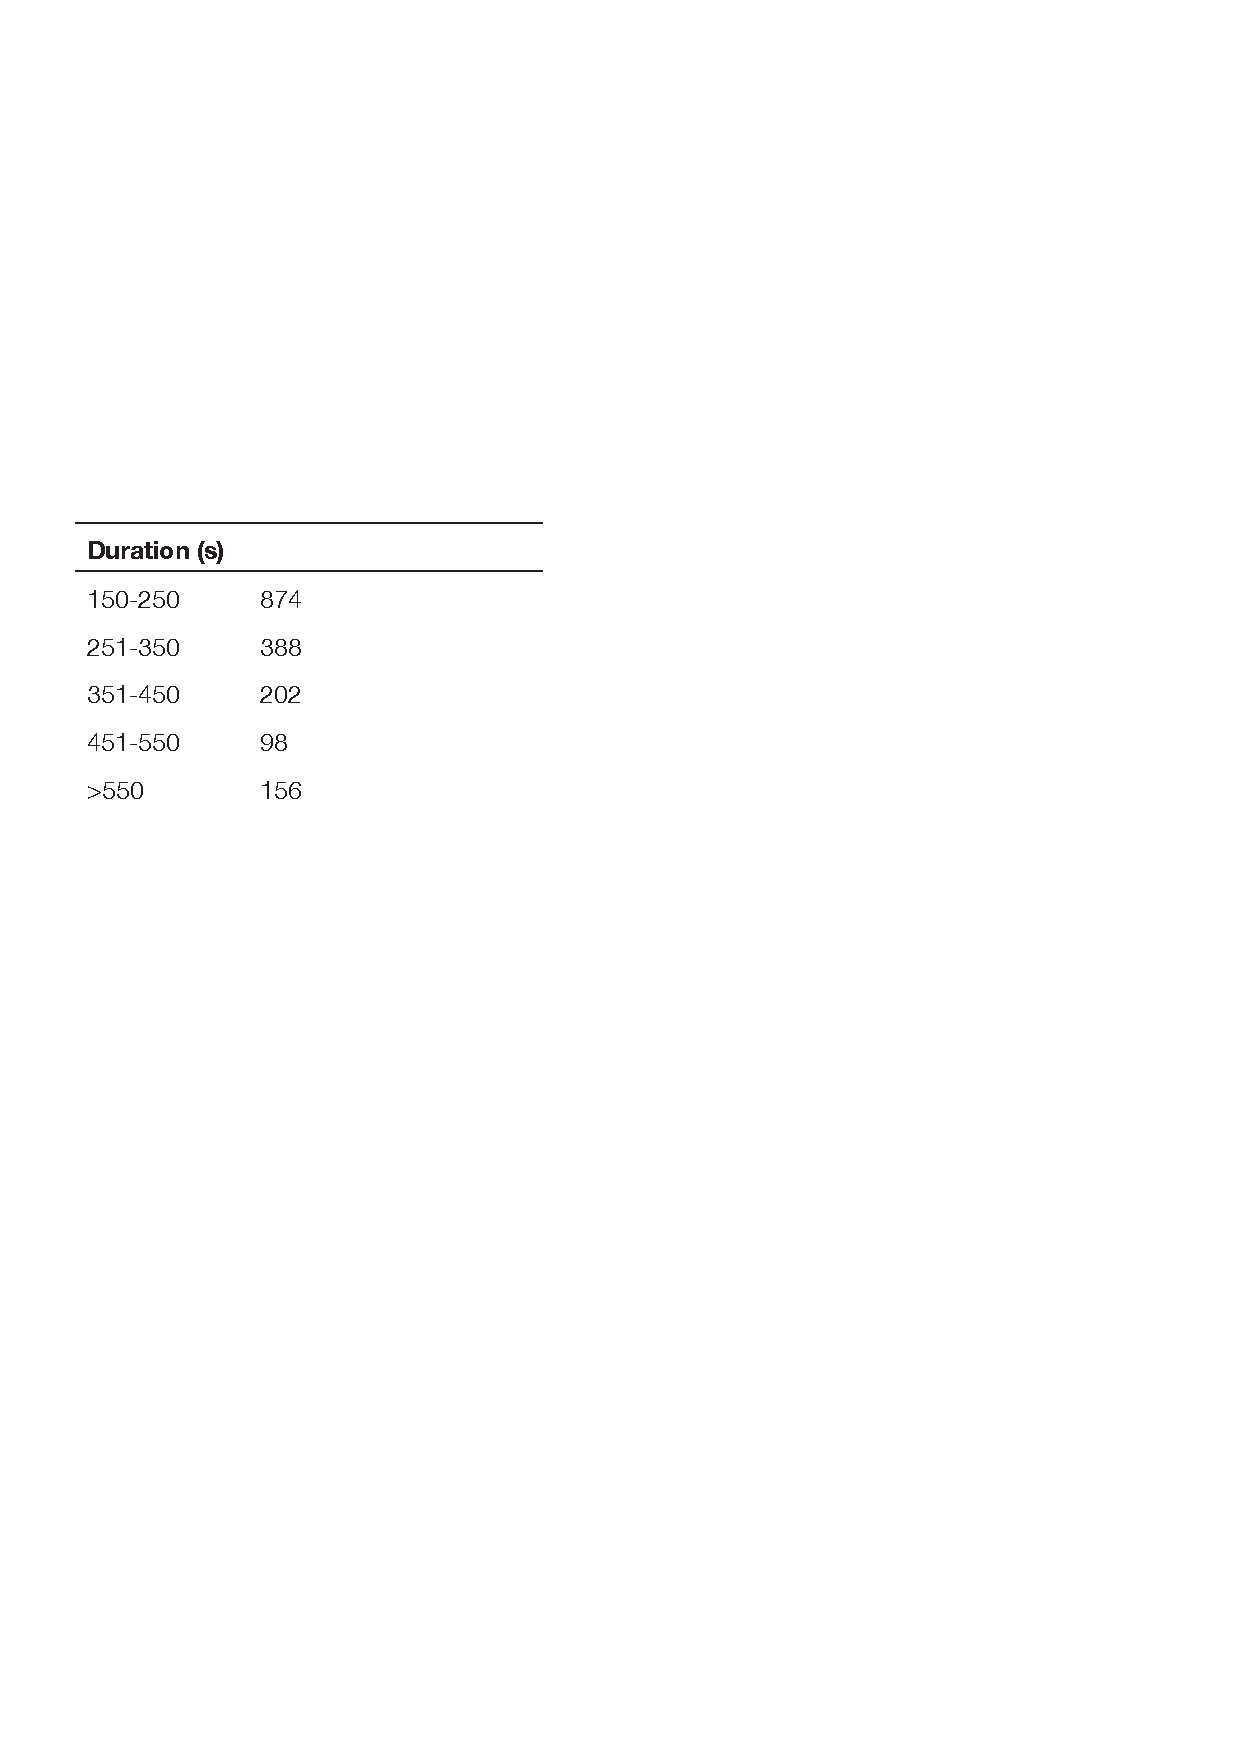
\includegraphics[scale=0.8]{images/ch56/ch56_LongWindowDurations.pdf}}
\caption[Study 7 frequency of long window durations]{Total number of occurrences that a window was in focus for longer than 150 seconds.}
\label{tbl:ch56-tblwindowdurations}
\end{table}

\begin{comment}
\begin{figure}
\centering
\centerline{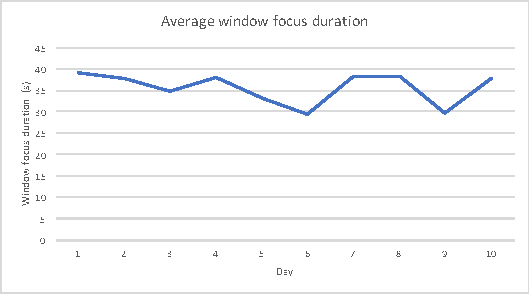
\includegraphics[scale=1]{images/ch56/ch56_MTDurationSwitches.pdf}}
\caption[Study 7 average window focus durations]{Average window focus durations during the study.}
\label{fig:ch56-7_mtdurswitches}
\end{figure}

\begin{figure}
\centering
\centerline{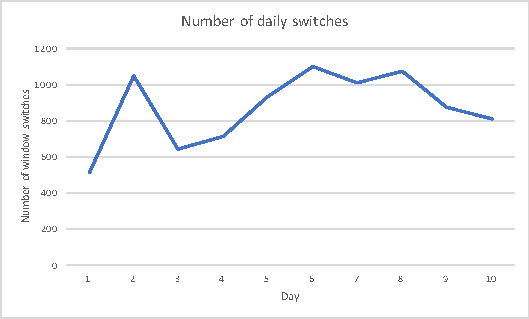
\includegraphics[scale=1]{images/ch56/ch56_MTNrSwitches.pdf}}
\caption[Study 7 average number of daily switches]{Average number of daily window switches during the study.}
\label{fig:ch56-7_mtnrswitches}
\end{figure}
\end{comment}

\subsubsection{Awareness of interruption behaviour}
Participants were largely aware they interrupted their work frequently and considered it the nature of their job: they regularly had to stop their work to look up task-related information, and had to address ad-hoc queries and requests from their department. The extension made participants realise however that they were unaware of the length of some of these interruptions. The average interruption time was considered much longer than they thought. 
Interview results suggest that common reasons for interruptions being longer than they thought were distractions and chains of diversion \citep{Hanrahan2015, Iqbal2007}, where the user further self-interrupts for other tasks. Participants tried to avoid interruptions during work that were completely unrelated, but after they had interrupted themselves for work purposes, there were opportunities to further self-interrupt for other off-task activities. The notification made people more aware of the effect this had on the duration of their interruptions:

\textit{"It's a shock, because I knew it was bad, I didn't think it was that bad. (…) So it's reflecting on, actually, a two-minute task is turning into a 15-20 minute task - why is that? (…) Why? But again, it's distractions."} (P9)

\textit{"It made me realise how long I was spending, spending/wasting, doing other stuff. (…)  It’s just going to do something and then ending up chatting with someone."} (P3)

\subsubsection{Reflecting on actions during an interruption}
The increased awareness of time spent on interruptions caused people to reflect on what they were doing during past interruptions. Some interruptions were urgent, important, or necessary to progress with work, and therefore hard to avoid altogether. However, reflecting on the exact actions during the interruptions made people realise that some interruptions could be shortened, as participants often ended up getting diverted from the original goal of the interruption. For example, upon switching to their email inbox to retrieve information, participants would get diverted by reading and responding to other unread messages instead. To help remember what was happening during an interruption, P9 combined the extension with the data of ManicTime: \textit{"[The extension] popped up and it said: ”You go away for 7 minutes and 33 seconds. I would then have a browse [in ManicTime] And then I think: oh my gosh, I've been on emails for an hour! I haven't got anything done. So yeah, I checked it quite a lot. More so because I was so shocked. And so, I'm so interested to know, actually, what I'm doing at work."} (P9)

Having this insight into their actions, participants tried to be more focused on the goal of subsequent interruptions and be more wary of potential distractions. It also happened that the duration of an interruption was considered long, but justified. P7 was the only participant who, upon viewing the time information, was not surprised by the time she spent on work-related interruptions. She considered the amount of time necessary to complete her work and did not see any room to improve on this: \textit{"To me, it doesn't kind of make me think: 'Oeh, I've been away too long'. I just think: OK, well I'm roughly aware that I've been away for an hour (…), I don't see how it kind of links with being more productive. Unless I suppose, you're really easily distracted."} (P7)

These findings show that awareness of time spent on interruptions can improve focus on the intention of interruption, and make people pay more attention to when they might get distracted. It also indicates that people may in particular benefit of feedback during interruptions where they are likely to get distracted, such as when switching to communication tools. 

\subsubsection{Reflecting on the relevance of interruptions}
Some work-related interruptions were not urgent, but participants were used to addressing them anyway if they were presumed to be ‘quick and easy’. These were addressed immediately so participants did not have to remind themselves to attend to it later, and it made them feel more productive if they completed more tasks. The notification made them more aware of the occurrence and actual length of these interruptions, and that they weren’t as quick as they thought. For future interruptions, people tried to consider whether they needed to address the interruption immediately:  \textit{"I need to work on time management and (…) not spending my whole day answering irrelevant queries."} (P9)

Participants mentioned several sources they knew to be distracting, such as email, their phone, and colleagues. Some sources of distraction were not essential for work, and generally participants did not self-interrupt their work often with the intention to access these sources: for example, several participants said they did not check social media at work. However, other distracting sources were used both for work and non-work purposes, such as search engines, instant messaging tools and email. It was therefore difficult to simply eliminate these distracting sources from the work environment:

\textit{"As everyone says, ‘we’ll just switch email off’ (…). But you can bet your life that there will come a moment in whatever task you’re doing you think: Oh! I have to open up email. And the moment you open up your email, that’s it."} (P2)

\textit{"My phone is a distraction for me. (…) I put my phone in a tray under a load of documents. But then (…) I converse a lot with a professor via text."} (P9)

This finding highlights the importance of giving people control over whether to address an interruption or not, as an interruption may be considered distracting but also essential for work. It demonstrates that an increased awareness of interruptions makes people reflect on why they interrupt and judge the relevance of the interruption, which may help in reducing unnecessary interruptions.

\subsubsection{Time information for task management and perceived productivity}
Completing tasks was an important component of people's work: they had an increased feeling of productivity if they explicitly ticked tasks off a list, and were driven by to-do lists and deadlines. While this could motivate people to focus on finishing a task before switching to another, it also had the contradicting effect that they interrupted their work often, if a task appeared that was considered easier to complete: 

\textit{"It kind of contradicts what I told you before about (…) how I jump on them [incoming tasks] and finish them. But at the same time, it’s because I don’t want to have three things at once going. I want to finish, finish, finish."} (P3)

The extension was started by the user deliberately selecting one window as a main task page, which forced participants to choose one task to focus on, and switching to other tasks was now considered an ‘interruption’ away from this task. As discussed earlier, the notification made people reflect more on whether other tasks they were switching to were relevant to address at that moment. 

A clear interest among participants was to not only see how much time they spent on interruptions away from the main task, but also how much time they spent on that main task overall. Currently, participants planned tasks they wanted to complete on either a daily or weekly basis, and implicitly took the time each task would take into consideration. However, given the fragmented nature of their role and the frequency of interruptions, it was difficult to estimate how long they actually spent on these tasks:

\textit{"I think that might take me 3 hours, and I’d want to get that done in one day. But yeah, obviously, things quite often take longer than I think I will, because then when I’m doing them, I might get interrupted."} (P5)

 In the same way that they used time information to reflect on whether interruptions were as long as they thought they were, they wanted to reflect on whether tasks took as long as expected. They would use this insight to be more realistic when planning tasks over time: 

\textit{"Down the line, I’d think it would be extremely useful to know how much time I’m actually spending [on tasks]. Because it would help me be more productive, or be more realistic in the amount of time I need for these things to happen."} (P3) 

These findings shows that both time away from a task, and time on a specific task, are important insights for workers to manage their work.

\subsubsection{Setting goals for time limits}
The notification was also used by participants to set goals on how much time they were willing to spend on interruptions. The way the notification was set up, participants did not know how much time they were spending on a specific interruption, and only saw the average interruption time. Therefore, several participants wanted to set time limits on each interruption. Similar to the relevance of an interruption, the appropriate length of an interruption was context-dependent as well: participants sometimes had to spend a relatively long time away from a task, for example if they had to find information in another window. It may therefore be more appropriate to give participants discretionary reminders to return to a task after they have reached a certain time limit, but then still give them control whether to adhere to that limit or not. Reaching the time limit could mean they were getting distracted, but it could also be the case that they were working on something relevant for work that needed more time: 

\textit{"Say you have to work on that specific document, and then you end up spending half an hour on Slack, chatting to your colleagues, it would be good if something's like: mate, work. Stop doing other things. But it’s really hard to know what people are actually doing on these things."} (P3)

These findings show that people need not only be in control of whether to address an interruption or not, but also for how long. They may however benefit from time information during an interruption to help them learn how to self-adjust their behaviour. 

\subsubsection{Context of information}
We asked participants about their use of the information provided by the extension versus ManicTime. Participants reported that the information provided by the extension was easy to read and interpret during a task. It was also clear what action to take, and participants used the information to decide whether they should reflect on past interruptions, and whether they could shorten the time away from their task. Participants looked at ManicTime at the start of the study out of curiosity and to make sure it was recording their activity correctly. However, in line with prior work \citep{Collins2014}, the extensiveness of the ManicTime data made it unclear to participants what action to take from the data, and most of them did not engage much with it for the rest of the study. It was considered too effortful and time-consuming to interpret and use the data:

\textit{"I didn’t go into too much detail with it. One of the reasons is that, it would take me a lot of time and effort to use this information, to help me work better or quicker, or more efficiently. And this is either something that I don’t have time to do, or I can’t be bothered, depending on the day."} (P3)

P9 did use ManicTime, in particular to help aid her reflection on what she was doing during past interruptions, a reflection which was triggered by the extension. 

Participants commented that they would have liked to be able to see additional information of their interruption behaviour over time, in addition to interruptions during the current task they were working on, to place into context whether their interruption length was higher or lower than their usual behaviour. They would use this information to set realistic goals on interruption lengths, and to see how often they were meeting these goals.
These findings show that short and actionable time information during a task can relieve users of the burden to interpret large amounts of information and easily adjust their behaviour. It also indicates that access to more information if needed is useful to get more insight into how people can change their behaviour, and whether they are achieving certain user goals. 

\subsubsection{Different work environments}
Seven participants worked from home on occasion, and saved up tasks that required focused attention to complete at home as the office was seen as a more distracting environment. There was an implicit understanding within their department that working from home meant they needed to concentrate, and as a result, participants received fewer interruptions caused by queries from colleagues:

\textit{"You’re working from home for a specific purpose, and therefore you don’t really want to be disturbed. Unless it’s absolutely urgent."} (P2) 

At the office, participants dealt with more interruptions taking place outside of the computer: for example, participants were interrupted by their colleagues or phone calls. Because the extension only provided time information about digital interruptions, some participants felt it provided an incomplete picture of their interruption behaviour. ManicTime provided participants with information on their non-digital interruptions, and participants considered this a good complement to the information that the extension provided. If the PC was inactive, and participants came back from inactivity, ManicTime presented users with a window on the screen saying how long they had been away for (see  Figure \ref{fig:ch56-7_mtaway}), and gave participants the option to write down what they had been doing while they were away.

The office environment not only exposed participants to more external interruptions, but participants also self-interrupted more in the office:
\textit{"From home it’s a bit different, I normally look at the emails but I generally try not to respond, unless it’s too urgent. But at work, when I’m here, (…) if it is not too urgent, but still I can find that is nice and straightforward, I just straight reply back. But at home it’s more focused, definitely."} (P8)

\textit{"When I’m at home, I generally don’t look at my phone for some weird reason. (…) When I’m in the office I find that I’m easily distracted, and I don’t get things done."} (P9)

All seven participants reported there were more sources to get distracted in the office. For example, most participants had multiple computer screens and kept the majority of documents, browse windows and applications open on their work computer, even after they had finished with them. These windows were a further source of distraction if participants were trying to find task-related information in one of the windows:

\textit{"It’s like 15 tabs, and I need to go somewhere. And I end up clicking all of them. And if there is one that is personal stuff, I end up reading it. And then five minutes after, I’m like: what was I doing? (…) So it’s distracting in the way that it makes me not solely focused on one thing."} (P3)

When working in the office, participants tried to complete tasks that required focused attention in the morning. They were more easily distracted in the afternoon, as they received more external interruptions, such as email, phone calls, and colleagues. These differences in work environments indicate that people get more easily distracted in some environments and at certain times. Though participants only used the extension in the office, their descriptions of their office and home environments indicate that participants may in particular benefit from time information during afternoon work in the office, when participants were more prone to interrupt themselves and get distracted.

\begin{figure}
\centering
\centerline{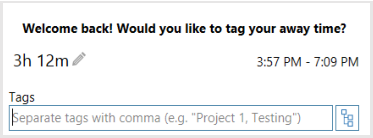
\includegraphics[scale=1]{images/ch56/ch56_MTaway.pdf}}
\caption[Study 7 ManicTime feedback on non-digital interruptions]{ If participants had been away from their computer, upon returning ManicTime presented them with a window showing how long they had been away for, and an option to write down what they had been doing while away.}
\label{fig:ch56-7_mtaway}
\end{figure}

\subsection{Discussion}
The aim of this study was to investigate whether showing people how long they go away from a task has an effect on their self-interruption behaviour during data entry work in an office sestting. The main finding is that time feedback made people reflect on what they were doing during interruptions. As a result, participants said they were more focused on the intention of an interruption, and wary of potential distractions and diversions from this intention. Having insight into the time they spent on interruptions tried to avoid interruptions that were not relevant, and set goals for how much time they were willing to spend on interruptions that were relevant. Some participants indicated that they would like to see time spent on a task as well, to help them schedule their tasks and improve their productivity. 

In line with previous work, the study indicates that an increased awareness of how people use time can improve focus on work \citep{Mark2018, Whittaker2016}. While previous work mainly found a reduction of time spent on non-work applications, a novel finding from the current study is that it can also benefit work-relevant interruptions: people shortened task-related interruptions to look up relevant information. 

The finding that people reflected on what they were doing during an interruption, as well as on the relevance of an interruption, is important as it suggests that people become more aware and in control of the intention of their interruptions. Prior work showed that self-interruptions can be beneficial, such as a break from work, as long as the interruption is triggered by a clear intention from the user, and not an unintended distraction \citep{Pang2016}. The results of the current study indicate that increased awareness of interruption behaviour may make interruptions more intentional, and reduce unintended diversions during these interruptions.

In addition to time away from a task, participants wanted to see information of time spent on a task. \citet{Whittaker2016}, who presented users with the last 30 minutes of their computer activity, found that giving people feedback on their use of time decreased the time spent away from work, but did not increase time on work, and speculated that people may have time limits to spend on work. Rather than increasing the amount of time spent on work, time feedback on task may be useful for people to better plan when and how they spend time on tasks. It may also make it even more apparent how interruptions slows down their work, as it is not only the time during an interruption, but also the resumption time after an interruption, that slows down work \citep{Altmann2004}. This effect was also demonstrated in Study 6, where people who made longer switches were slower to complete a task, even after removing the duration times. 

Participants were more distracted in the office in the afternoon, which is in line with \citet{Mark2014} who found that boredom in the workplace is highest in the afternoon, and people are more likely to self-interrupt when they are bored. A further likely reason found in the current study was that it was busier in the office in the afternoon, and participants were exposed to more external interruptions: prior research found that an increase in external interruptions leads to more self-interruptions \citep{Dabbish2011}. In contrast, participants who worked from home said they were more focused at home and experienced fewer interruptions. This means that people may in particular benefit from time information at certain moments and settings, when people are more likely to get distracted. Participants only used the extension at the office and it is therefore unclear whether they would use it differently when working from home. Future research could further investigate people's self-interruption behaviour in different work settings. 

Interruptions can have both benefits and costs, and it is important to consider the properties that make an interruption disruptive. The study highlights that whether or not to address an interruption, and for how long, not only depends on interruption properties but also the context in which an interruption occurs. For instance, email may be considered distracting and is best avoided in some situations, but in another situation the user may need to find information in email which is essential for the current task. Furthermore, the longer people interrupt a task, the more disruptive it is \citep{Altmann2017, Monk2008}, but in some situations it is important to find information and spend this time away from a task. Prior approaches to block self-interruptions to distracting sources \citep{Kim2017, Mark2018} or impose time limits \citep{Freedom} are too restrictive in this situation. A more appropriate approach is to give users control to decide when and how long to address interruptions, and give them useful information to help them learn how to best control and self-adjust their behaviour. This echoes earlier conclusions by \citet{Mark2018} who found that blocking distractions at the workplace was experienced by several participants as too controlling, and participants rather wanted to learn to gain control of their work. The studies make an important contribution by showing how showing people feedback on interruption length can help in gaining control over time spent on interruptions. 

\subsubsection{Implications for design}
Previous work has highlighted several problems with existing commercial time tracking and management applications: these often are time-consuming to use, they can restrict user activities too much, and it is not immediately clear to users what action to take based on the data \citep{Collins2014, Whittaker2016}. The findings from the current study partly corroborate these issues, and demonstrate several pointers that can inform the design of time applications. 

\textit{Complement time information}. First, when providing users with a data log of their computer activities, they need to have a specific starting point of what it is they want to find out for them to be able to use it and act on it. Participants were not interested in their overall computer activity, but were mostly interested in the time they spent on, or away from, a specific task. By presenting a simple and precise measure, namely the length of an interruption, participants were provided with a specific target of what to reflect on and change, and did not need to go through the effort of having to interpret information of all their activity. As some participants did want to have access to more detailed information about their activity during a specific interruption, a simple presentation in the moment can be complemented by a more complete log running in the background. It would also be interesting to give users control over what information they are interested in to see in the notification. For example, most participants were not only interested in the length of interruptions during a task, but also on the length of their task overall. This could help participants to better manage their tasks.

\textit{Time feedback during a task}. Second, by showing information during the task, participants can react and change their behaviour immediately and do not have to remind themselves to look at information later \citep{Gould2016, Maior2018}. Participants were prompted by the notification to reflect on what they were doing during an interruption, but often forgot to look back at their computer activities on other occasions. Furthermore, participants in Study 6 were able to act on the explicit information they were given in the short time space of an experiment, which had a positive effect on their task performance.

\textit{Setting time limits and time goals}. Several participants wanted to set time limits on interruptions, which has also been found in earlier work on interruptions \citep{Mark2018, Whittaker2016}. Based on the finding however that interruptions are context-dependent, imposing a strict time limit may be too restrictive. Rather, giving timed reminders to return to a task may make people more aware of the length of their interruptions, while still giving them control whether to actually return to a task or not. 

\textit{Behaviour over time}. Lastly, a promising area to investigate would be to record the interruptions and give participants insight in how their changes have an effect over time. Although it was clear to participants what action they had to take based on the data presented by the extension, some felt they did not have sufficient information as to whether their changes had any effect over time.

\subsubsection{Limitations}
While the results are promising, the study also has a number of limitations which would be worthwhile to address in future work. The notification only provides feedback on digital interruptions, but as was apparent both in Study 2 and Study 7, people also deal with interruptions and distractions beyond the computer. Future work could look at also collecting and showing data from these interruptions. For example, ManicTime uses PC inactivity to indicate when participants were away. Other sensitive measures to detect moments where the user has likely interrupted their work could be inter-key intervals or mouse clicks. Furthermore, due to the limited logging data, it is difficult to make any concluding claims as to whether time feedback had any significant effect on participants’ window switching and task focus behaviour over time. In addition, though participants indicated they modified their behaviour after using the extension, it is not certain whether they based their behaviour on the specific information provided by the extension, or whether the notification simply made them reflect and become more aware of their time. 

\section{Summary of Chapter 5}
The aim of this chapter was to investigate whether showing people how long they go away from a task has an effect on their self-interruption behaviour. The findings demonstrate that time feedback can reduce distractions and improve task performance. Study 6 showed that it reduced the duration of switches, made people faster in completing a data entry task and reduced data entry errors. Study 7 showed that time feedback made people reflect on what they were doing during an interruption. They avoided interruptions that were not relevant, and set goals for how much time they were willing to spend on interruptions that were relevant. They were more focused on the intention of an interruption, and wary of potential distractions and diversions from this intention. 

The studies presented in this chapter contribute to our understanding of switching behaviour for routine data entry work to distracting but task-relevant applications such as email. The results suggest that a simple presentation of time information during a task can mitigate distractions but still keep users in control over their interruptions, and can inform the design of productivity interventions to improve focus. Showing users how long they go away from a task can increase awareness of interruption behaviour, which can reduce the duration of interruptions, shorten the completion time of tasks and reduce errors.

The next chapter brings together the findings from all studies, and further discusses the practical implications and the contributions that the findings make to knowledge. It also discusses opportunities for future work.